% Options for packages loaded elsewhere
\PassOptionsToPackage{unicode}{hyperref}
\PassOptionsToPackage{hyphens}{url}
%
\documentclass[
]{book}
\usepackage{amsmath,amssymb}
\usepackage{lmodern}
\usepackage{iftex}
\ifPDFTeX
  \usepackage[T1]{fontenc}
  \usepackage[utf8]{inputenc}
  \usepackage{textcomp} % provide euro and other symbols
\else % if luatex or xetex
  \usepackage{unicode-math}
  \defaultfontfeatures{Scale=MatchLowercase}
  \defaultfontfeatures[\rmfamily]{Ligatures=TeX,Scale=1}
\fi
% Use upquote if available, for straight quotes in verbatim environments
\IfFileExists{upquote.sty}{\usepackage{upquote}}{}
\IfFileExists{microtype.sty}{% use microtype if available
  \usepackage[]{microtype}
  \UseMicrotypeSet[protrusion]{basicmath} % disable protrusion for tt fonts
}{}
\makeatletter
\@ifundefined{KOMAClassName}{% if non-KOMA class
  \IfFileExists{parskip.sty}{%
    \usepackage{parskip}
  }{% else
    \setlength{\parindent}{0pt}
    \setlength{\parskip}{6pt plus 2pt minus 1pt}}
}{% if KOMA class
  \KOMAoptions{parskip=half}}
\makeatother
\usepackage{xcolor}
\usepackage[margin=1in]{geometry}
\usepackage{color}
\usepackage{fancyvrb}
\newcommand{\VerbBar}{|}
\newcommand{\VERB}{\Verb[commandchars=\\\{\}]}
\DefineVerbatimEnvironment{Highlighting}{Verbatim}{commandchars=\\\{\}}
% Add ',fontsize=\small' for more characters per line
\usepackage{framed}
\definecolor{shadecolor}{RGB}{248,248,248}
\newenvironment{Shaded}{\begin{snugshade}}{\end{snugshade}}
\newcommand{\AlertTok}[1]{\textcolor[rgb]{0.94,0.16,0.16}{#1}}
\newcommand{\AnnotationTok}[1]{\textcolor[rgb]{0.56,0.35,0.01}{\textbf{\textit{#1}}}}
\newcommand{\AttributeTok}[1]{\textcolor[rgb]{0.77,0.63,0.00}{#1}}
\newcommand{\BaseNTok}[1]{\textcolor[rgb]{0.00,0.00,0.81}{#1}}
\newcommand{\BuiltInTok}[1]{#1}
\newcommand{\CharTok}[1]{\textcolor[rgb]{0.31,0.60,0.02}{#1}}
\newcommand{\CommentTok}[1]{\textcolor[rgb]{0.56,0.35,0.01}{\textit{#1}}}
\newcommand{\CommentVarTok}[1]{\textcolor[rgb]{0.56,0.35,0.01}{\textbf{\textit{#1}}}}
\newcommand{\ConstantTok}[1]{\textcolor[rgb]{0.00,0.00,0.00}{#1}}
\newcommand{\ControlFlowTok}[1]{\textcolor[rgb]{0.13,0.29,0.53}{\textbf{#1}}}
\newcommand{\DataTypeTok}[1]{\textcolor[rgb]{0.13,0.29,0.53}{#1}}
\newcommand{\DecValTok}[1]{\textcolor[rgb]{0.00,0.00,0.81}{#1}}
\newcommand{\DocumentationTok}[1]{\textcolor[rgb]{0.56,0.35,0.01}{\textbf{\textit{#1}}}}
\newcommand{\ErrorTok}[1]{\textcolor[rgb]{0.64,0.00,0.00}{\textbf{#1}}}
\newcommand{\ExtensionTok}[1]{#1}
\newcommand{\FloatTok}[1]{\textcolor[rgb]{0.00,0.00,0.81}{#1}}
\newcommand{\FunctionTok}[1]{\textcolor[rgb]{0.00,0.00,0.00}{#1}}
\newcommand{\ImportTok}[1]{#1}
\newcommand{\InformationTok}[1]{\textcolor[rgb]{0.56,0.35,0.01}{\textbf{\textit{#1}}}}
\newcommand{\KeywordTok}[1]{\textcolor[rgb]{0.13,0.29,0.53}{\textbf{#1}}}
\newcommand{\NormalTok}[1]{#1}
\newcommand{\OperatorTok}[1]{\textcolor[rgb]{0.81,0.36,0.00}{\textbf{#1}}}
\newcommand{\OtherTok}[1]{\textcolor[rgb]{0.56,0.35,0.01}{#1}}
\newcommand{\PreprocessorTok}[1]{\textcolor[rgb]{0.56,0.35,0.01}{\textit{#1}}}
\newcommand{\RegionMarkerTok}[1]{#1}
\newcommand{\SpecialCharTok}[1]{\textcolor[rgb]{0.00,0.00,0.00}{#1}}
\newcommand{\SpecialStringTok}[1]{\textcolor[rgb]{0.31,0.60,0.02}{#1}}
\newcommand{\StringTok}[1]{\textcolor[rgb]{0.31,0.60,0.02}{#1}}
\newcommand{\VariableTok}[1]{\textcolor[rgb]{0.00,0.00,0.00}{#1}}
\newcommand{\VerbatimStringTok}[1]{\textcolor[rgb]{0.31,0.60,0.02}{#1}}
\newcommand{\WarningTok}[1]{\textcolor[rgb]{0.56,0.35,0.01}{\textbf{\textit{#1}}}}
\usepackage{longtable,booktabs,array}
\usepackage{calc} % for calculating minipage widths
% Correct order of tables after \paragraph or \subparagraph
\usepackage{etoolbox}
\makeatletter
\patchcmd\longtable{\par}{\if@noskipsec\mbox{}\fi\par}{}{}
\makeatother
% Allow footnotes in longtable head/foot
\IfFileExists{footnotehyper.sty}{\usepackage{footnotehyper}}{\usepackage{footnote}}
\makesavenoteenv{longtable}
\usepackage{graphicx}
\makeatletter
\def\maxwidth{\ifdim\Gin@nat@width>\linewidth\linewidth\else\Gin@nat@width\fi}
\def\maxheight{\ifdim\Gin@nat@height>\textheight\textheight\else\Gin@nat@height\fi}
\makeatother
% Scale images if necessary, so that they will not overflow the page
% margins by default, and it is still possible to overwrite the defaults
% using explicit options in \includegraphics[width, height, ...]{}
\setkeys{Gin}{width=\maxwidth,height=\maxheight,keepaspectratio}
% Set default figure placement to htbp
\makeatletter
\def\fps@figure{htbp}
\makeatother
\setlength{\emergencystretch}{3em} % prevent overfull lines
\providecommand{\tightlist}{%
  \setlength{\itemsep}{0pt}\setlength{\parskip}{0pt}}
\setcounter{secnumdepth}{5}
\usepackage{booktabs}
\ifLuaTeX
  \usepackage{selnolig}  % disable illegal ligatures
\fi
\usepackage[]{natbib}
\bibliographystyle{apalike}
\IfFileExists{bookmark.sty}{\usepackage{bookmark}}{\usepackage{hyperref}}
\IfFileExists{xurl.sty}{\usepackage{xurl}}{} % add URL line breaks if available
\urlstyle{same} % disable monospaced font for URLs
\hypersetup{
  pdftitle={Becoming Fluent in Data},
  pdfauthor={Marco Kühne},
  hidelinks,
  pdfcreator={LaTeX via pandoc}}

\title{Becoming Fluent in Data}
\usepackage{etoolbox}
\makeatletter
\providecommand{\subtitle}[1]{% add subtitle to \maketitle
  \apptocmd{\@title}{\par {\large #1 \par}}{}{}
}
\makeatother
\subtitle{Empirical Research (with R) -- Based On True Stories}
\author{Marco Kühne}
\date{2022-08-23}

\begin{document}
\maketitle

{
\setcounter{tocdepth}{1}
\tableofcontents
}
\hypertarget{dust-and-dark}{%
\chapter*{Dust and Dark}\label{dust-and-dark}}
\addcontentsline{toc}{chapter}{Dust and Dark}

A dusty lecture hall. The light cut through the darkness from the left side of the room. A dozen of seats in each bench, only few occupied by small groups of students who were trying to make sure that they sit far from each other and as far as possible from the lecturer. The bearish but competent assistant professor explained how to analyze and evaluate the results of various memory and cognition experiments through boxplots, t-test and the like in that software. My creaky, slow but loyal laptop in front of me. That's where R was introduced in my psychology undergraduate studies.

\begin{infobox2}warning

\begin{itemize}
\tightlist
\item
  Conceptual Skills: What makes a good comparison. Never use pie charts.
\item
  Data Skills:

  \begin{itemize}
  \tightlist
  \item
    R Basics: Install and load a package. Load Stata files into R.
  \item
    Data Manipulation: \texttt{tidyverse} language (\texttt{glimpse()}, \texttt{count()}, \texttt{filter()}, \texttt{summarise()}).
  \item
    Data Visualization: Pie chart and bar plot.
  \end{itemize}
\end{itemize}

\end{infobox2}

\hypertarget{part-preface}{%
\part{Preface}\label{part-preface}}

\hypertarget{teach-learn-repeat}{%
\chapter*{Teach -- Learn -- Repeat}\label{teach-learn-repeat}}
\addcontentsline{toc}{chapter}{Teach -- Learn -- Repeat}

I fell in love with \href{https://en.wikipedia.org/wiki/Learning_by_teaching}{learning by teaching} the moment I came across this concept. It put the experiences I made into scientific context. I had to pass math classes in my undergraduates, and I became a math tutor for years. I really wanted to master ballroom dance, so I became a dance instructor for life.

The mode of teaching can differ. I started teaching in the classroom and ballroom and have a standing on Wikipedia. You can contribute on Wikipedia and will get feedback on your neutral point of view, academic writing and rigor. Feedback on YouTube and Social Media can be more diffuse. Now, I turn to writing a book from my collected notes (and questions) on empirical research. I hope to force myself to pinpoint exactly what I know and don't know and how to fill the gaps. Luckily, I am not alone with the approach of creating classes or writing books to learn.

\begin{quote}
I could feel that econometrics was indispensable, and yet I was missing something. But what? It was a theory of causality {[}\ldots{]}. So, desperate, I did what I always do when I want to learn something new --- I developed a course on causality to force myself to learn all the things I didn't know.

\hfill Scott Cunningham. In: Causal Inference -- The Mixtape
\end{quote}

This project helped me to learn more about R, RStudio, R Markdown, R Bookdown, HTML/CSS, Git and Github, empirical research, causal inference, statistics, math, frustration tolerance and fun.

\hypertarget{a-question-you-care-about}{%
\chapter*{A Question You Care About}\label{a-question-you-care-about}}
\addcontentsline{toc}{chapter}{A Question You Care About}

Are you passionate about something? Research starts off from a question you really care about. Math, statistics and programming are easier to digest when you are intrinsically motivated to find out more about your topic of interest. This is a brief guide on the main parts of the empirical research process. There's more to the end of it. After answering the research question, a theoretical interpretation can be derived, results are compared to earlier research and conclusions are drawn.

Give it a personal touch if possible. The topic can be related to hobbies, family or friends, education, job or neighborhood. It can be something from the present or past. It can be a pet as well as personality, believes and attitudes. It can be gardening or Fortnite. Choose something that you are really interested in. Next, retain a neutral point of view. Collect and analyze data first, discuss and compare your results to others, conclude at the end.

\includegraphics{Becoming-Fluent-In-Data_files/figure-latex/unnamed-chunk-1-1.pdf}

\begin{infobox}warning

What you can learn \ldots{}

\begin{itemize}
\tightlist
\item
  What is at the heart of empirical research: Questions.
\item
  How to get and handle tabular data.
\item
  The principles of relationships and trends.
\item
  How to model relationships with equations.
\item
  Estimate a relationship with Regression.
\item
  The implementation in the statistical software R.
\end{itemize}

\end{infobox}

\hypertarget{data-is-everywhere}{%
\chapter*{Data is everywhere}\label{data-is-everywhere}}
\addcontentsline{toc}{chapter}{Data is everywhere}

Data collection is the process of gathering and measuring information.

\hypertarget{methods}{%
\section*{Methods}\label{methods}}
\addcontentsline{toc}{section}{Methods}

There are common data collection methods:

\begin{itemize}
\tightlist
\item
  Surveys (paper vs.~online)
\item
  Interviews
\item
  Observation
\item
  Experiment
\item
  Focus group (qualitative research)
\item
  Case study (qualitative research)
\end{itemize}

\hypertarget{types-of-data}{%
\section*{Types of Data}\label{types-of-data}}
\addcontentsline{toc}{section}{Types of Data}

\begin{itemize}
\tightlist
\item
  Quantitative vs qualitative
\end{itemize}

Quantitative data deals with things that are measurable and can be expressed in numbers or figures, or using other values that express quantity. That being said, quantitative data is usually expressed in numerical form and can represent size, length, duration, amount, price, and so on.

Qualitative data is often non-numeric. Data can be text, audio or visual. There are quantitative approaches to analyse text (text mining, e.g.~sentiment analysis) and visual data (machine learning, e.g.~image classification).

\begin{itemize}
\tightlist
\item
  Primary vs secondary
\end{itemize}

\emph{Primary data} refers to the first hand data gathered by the researcher or practitioner himself.

\emph{Secondary data} means data collected by someone else earlier.

As you expect, it can be more complicated, cost and time expensive to collect data yourself.

\begin{itemize}
\tightlist
\item
  Cross-sectional vs.~longitudinal data
\end{itemize}

Cross-sectional data is at a point in time (e.g.~one year).

Longitudinal data is repeated measures over time (e.g.~multiple years). Also called panel data.

\hypertarget{intro-to-r}{%
\chapter*{Intro to R}\label{intro-to-r}}
\addcontentsline{toc}{chapter}{Intro to R}

An .R file is a text document. Open (and edit) it with a any text editor (or RStudio). Comments start with one or multiple hash tags.

\hypertarget{watching-paint-dry}{%
\section*{Watching paint dry}\label{watching-paint-dry}}
\addcontentsline{toc}{section}{Watching paint dry}

Use this R demo in the browser to explore basic features of R. Copy commands from lower sections, paste them into \textbf{script.R} and hit the \textbf{Run} bottom. It runs the entire script and prints out results in the \textbf{R Console}. This procedure is simplified but similar to a more complex integrated developer environment (IDE) like RStudio.

eyJsYW5ndWFnZSI6InIiLCJzYW1wbGUiOiIjIENvbW1lbnQ6IFIgYXMgYSBjYWxjdWxhdG9yIGlzIGEgYm9yaW5nIGFzIHdhdGNoaW5nIHBhaW50IGRyeS5cbjIxKjIgIn0=

Try \texttt{1:20} and hit Run.

\hypertarget{define-objects}{%
\section*{Define objects}\label{define-objects}}
\addcontentsline{toc}{section}{Define objects}

Define R objects for later use. Objects are \textbf{case-sensitive} (\texttt{X} is different from \texttt{x}). Objects can take any name, but its best to use something that makes sense to you, and will likely make sense to others who may read your code.

\hypertarget{numeric-variables}{%
\subsection*{Numeric Variables}\label{numeric-variables}}
\addcontentsline{toc}{subsection}{Numeric Variables}

\begin{Shaded}
\begin{Highlighting}[]
\NormalTok{a }\OtherTok{\textless{}{-}} \DecValTok{2}
\NormalTok{b }\OtherTok{=} \DecValTok{3}
\NormalTok{a }\SpecialCharTok{+}\NormalTok{ b}
\DocumentationTok{\#\# [1] 5}
\end{Highlighting}
\end{Shaded}

\hypertarget{logical-variables}{%
\subsection*{Logical Variables}\label{logical-variables}}
\addcontentsline{toc}{subsection}{Logical Variables}

\begin{Shaded}
\begin{Highlighting}[]
\SpecialCharTok{\textgreater{}}\NormalTok{ harvard               }\OtherTok{\textless{}{-}}        \ConstantTok{TRUE} \CommentTok{\# spacing doesn\textquotesingle{}t matter}
\SpecialCharTok{\textgreater{}}\NormalTok{ yale      }\OtherTok{\textless{}{-}} \ConstantTok{FALSE}
\SpecialCharTok{\textgreater{}}\NormalTok{ princeton }\OtherTok{\textless{}{-}}\NormalTok{ F }\CommentTok{\# short for FALSE}
\SpecialCharTok{\textgreater{}} 
\ErrorTok{\textgreater{}} \CommentTok{\# Attention: FALSE=0, TRUE=1}
\ErrorTok{\textgreater{}}\NormalTok{ harvard }\SpecialCharTok{+} \DecValTok{1}
\DocumentationTok{\#\# [1] 2}
\end{Highlighting}
\end{Shaded}

\hypertarget{string-variables}{%
\subsection*{String Variables}\label{string-variables}}
\addcontentsline{toc}{subsection}{String Variables}

\begin{Shaded}
\begin{Highlighting}[]
\NormalTok{emily  }\OtherTok{\textless{}{-}} \StringTok{\textquotesingle{}She is a friend.\textquotesingle{}}     \CommentTok{\# string / character class / plain text}
\NormalTok{libby  }\OtherTok{\textless{}{-}} \StringTok{"she is a coworker"}    \CommentTok{\# use \textquotesingle{} and " interchangeably}
\NormalTok{other  }\OtherTok{\textless{}{-}} \StringTok{"people"}               \CommentTok{\# prefer "}
\end{Highlighting}
\end{Shaded}

\hypertarget{factor-variables}{%
\subsection*{Factor Variables}\label{factor-variables}}
\addcontentsline{toc}{subsection}{Factor Variables}

A factor is an ordered categorical variable. \texttt{c()} is a generic function which combines its arguments.

\begin{Shaded}
\begin{Highlighting}[]
\NormalTok{fruit  }\OtherTok{\textless{}{-}} \FunctionTok{as.factor}\NormalTok{(}\FunctionTok{c}\NormalTok{(}\StringTok{"banana"}\NormalTok{, }\StringTok{"apple"}\NormalTok{)  ) }\CommentTok{\# The default ordering is alphabetic}
\NormalTok{fruit}
\end{Highlighting}
\end{Shaded}

\begin{verbatim}
## [1] banana apple 
## Levels: apple banana
\end{verbatim}

\begin{Shaded}
\begin{Highlighting}[]
\NormalTok{dose }\OtherTok{\textless{}{-}} \FunctionTok{as.factor}\NormalTok{(}\FunctionTok{c}\NormalTok{(}\StringTok{"low"}\NormalTok{, }\StringTok{"medium"}\NormalTok{, }\StringTok{"high"}\NormalTok{)  ) }\CommentTok{\# The default ordering is alphabetic}
\NormalTok{dose}
\end{Highlighting}
\end{Shaded}

\begin{verbatim}
## [1] low    medium high  
## Levels: high low medium
\end{verbatim}

\hypertarget{combine-objects}{%
\subsection*{Combine objects}\label{combine-objects}}
\addcontentsline{toc}{subsection}{Combine objects}

\begin{Shaded}
\begin{Highlighting}[]
\CommentTok{\# Declare new objects using other variables}
\NormalTok{c }\OtherTok{\textless{}{-}}\NormalTok{ a }\SpecialCharTok{+}\NormalTok{ b }\SpecialCharTok{+} \DecValTok{10}

\CommentTok{\# Open z object or put everything in parentheses}
\NormalTok{(c }\OtherTok{\textless{}{-}}\NormalTok{ a }\SpecialCharTok{+}\NormalTok{ b }\SpecialCharTok{+} \DecValTok{10}\NormalTok{)}
\end{Highlighting}
\end{Shaded}

\begin{verbatim}
## [1] 15
\end{verbatim}

\hypertarget{vectors}{%
\subsection*{Vectors}\label{vectors}}
\addcontentsline{toc}{subsection}{Vectors}

Think of a vector as a single column in a spreadsheet.

\begin{Shaded}
\begin{Highlighting}[]
\NormalTok{vectorA }\OtherTok{\textless{}{-}} \FunctionTok{c}\NormalTok{(}\DecValTok{1}\NormalTok{,}\DecValTok{2}\NormalTok{,b)}
\NormalTok{vectorB }\OtherTok{\textless{}{-}} \FunctionTok{c}\NormalTok{(}\ConstantTok{TRUE}\NormalTok{,}\ConstantTok{TRUE}\NormalTok{,}\ConstantTok{FALSE}\NormalTok{)}
\NormalTok{vectorC }\OtherTok{\textless{}{-}} \FunctionTok{c}\NormalTok{(emily, libby, other) }

\CommentTok{\# Vector Operations}
\NormalTok{vectorA }\SpecialCharTok{{-}}\NormalTok{ vectorB }\CommentTok{\# Vector operation AND auto{-}change TRUE =1, FALSE=0}
\end{Highlighting}
\end{Shaded}

\begin{verbatim}
## [1] 0 1 3
\end{verbatim}

\hypertarget{data-frame}{%
\subsection*{Data frame}\label{data-frame}}
\addcontentsline{toc}{subsection}{Data frame}

\begin{Shaded}
\begin{Highlighting}[]
\CommentTok{\# think of it conceptually like a spreadsheet}
\NormalTok{dataDF }\OtherTok{\textless{}{-}} \FunctionTok{data.frame}\NormalTok{(}\AttributeTok{numberVec    =}\NormalTok{ vectorA,}
                     \AttributeTok{trueFalseVec =}\NormalTok{ vectorB,}
                     \AttributeTok{stringsVec   =}\NormalTok{ vectorC)}

\CommentTok{\# Examine an entire data frame  }
\NormalTok{dataDF}
\end{Highlighting}
\end{Shaded}

\begin{verbatim}
##   numberVec trueFalseVec        stringsVec
## 1         1         TRUE  She is a friend.
## 2         2         TRUE she is a coworker
## 3         3        FALSE            people
\end{verbatim}

\begin{Shaded}
\begin{Highlighting}[]
\CommentTok{\# Declare a new column}
\NormalTok{dataDF}\SpecialCharTok{$}\NormalTok{NewCol }\OtherTok{\textless{}{-}} \FunctionTok{c}\NormalTok{(}\DecValTok{10}\NormalTok{,}\DecValTok{9}\NormalTok{,}\DecValTok{8}\NormalTok{)}

\CommentTok{\# Examine with new column}
\NormalTok{dataDF}
\end{Highlighting}
\end{Shaded}

\begin{verbatim}
##   numberVec trueFalseVec        stringsVec NewCol
## 1         1         TRUE  She is a friend.     10
## 2         2         TRUE she is a coworker      9
## 3         3        FALSE            people      8
\end{verbatim}

\begin{Shaded}
\begin{Highlighting}[]
\CommentTok{\# Examine a single column}
\NormalTok{dataDF}\SpecialCharTok{$}\NormalTok{numberVec }\CommentTok{\# by name}
\end{Highlighting}
\end{Shaded}

\begin{verbatim}
## [1] 1 2 3
\end{verbatim}

\begin{Shaded}
\begin{Highlighting}[]
\NormalTok{dataDF[,}\DecValTok{1}\NormalTok{] }\CommentTok{\# by index...remember ROWS then COLUMNS}
\end{Highlighting}
\end{Shaded}

\begin{verbatim}
## [1] 1 2 3
\end{verbatim}

\begin{Shaded}
\begin{Highlighting}[]
\CommentTok{\# Examine a single row}
\NormalTok{dataDF[}\DecValTok{2}\NormalTok{,] }\CommentTok{\# by index position}
\end{Highlighting}
\end{Shaded}

\begin{verbatim}
##   numberVec trueFalseVec        stringsVec NewCol
## 2         2         TRUE she is a coworker      9
\end{verbatim}

\begin{Shaded}
\begin{Highlighting}[]
\CommentTok{\# Examine a single value}
\NormalTok{dataDF}\SpecialCharTok{$}\NormalTok{numberVec[}\DecValTok{2}\NormalTok{] }\CommentTok{\# column name, then position (2)}
\end{Highlighting}
\end{Shaded}

\begin{verbatim}
## [1] 2
\end{verbatim}

\begin{Shaded}
\begin{Highlighting}[]
\NormalTok{dataDF[}\DecValTok{1}\NormalTok{,}\DecValTok{2}\NormalTok{] }\CommentTok{\#by index row 1, column 2}
\end{Highlighting}
\end{Shaded}

\begin{verbatim}
## [1] TRUE
\end{verbatim}

\hypertarget{plots}{%
\subsection*{Plots}\label{plots}}
\addcontentsline{toc}{subsection}{Plots}

\hypertarget{about-the-author}{%
\chapter*{About the author}\label{about-the-author}}
\addcontentsline{toc}{chapter}{About the author}

Welcome! My name is Marco Kühne (\url{http://marco-kuehne.com/}). The very first thing I want to do is to invite you to call me Marco. That is, if we meet on the street, you come talk to me during office hours, you ask some question; Marco's the name that I respond to.

I am a PhD candidate in Economics at the European University Viadrina (\url{https://www.wiwi.europa-uni.de/}). I am generally keen on teaching topics related to research design, quantitative methods, and statistical software. My main methodological interests in quantitative social science include panel data modelling, causal inference with observational data and R programming.

I am also a gardening fanatic, a coffee enthusiast, an engaged ballroom dancer, a (vegetarian) food lover. I enjoy cutting down big trees and practicing new languages in its own sake. Feel free to contact me!

\begin{figure}

{\centering \includegraphics[width=0.6\linewidth]{images/Marco-scaled} 

}

\caption{\label{fig:figs}plotting example}\label{fig:unnamed-chunk-13}
\end{figure}

\hypertarget{part-data-analysis}{%
\part{Data Analysis}\label{part-data-analysis}}

\hypertarget{group-comparison}{%
\chapter{Group Comparison}\label{group-comparison}}

In this section you learn about how to compare groups.

\hypertarget{learning-goals}{%
\section{Learning Goals}\label{learning-goals}}

\begin{infobox2}warning

\begin{itemize}
\tightlist
\item
  Conceptual Skills: What makes a good comparison. Never use pie charts.
\item
  Data Skills:

  \begin{itemize}
  \tightlist
  \item
    R Basics: Install and load a package. Load Stata files into R.
  \item
    Data Manipulation: \texttt{tidyverse} language (\texttt{glimpse()}, \texttt{count()}, \texttt{filter()}, \texttt{summarise()}).
  \item
    Data Visualization: Pie chart and bar plot.
  \end{itemize}
\end{itemize}

\end{infobox2}

Social sciences is about the study of human beings and their interactions. As such, we frequently want to compare two or more groups of human beings, organizations, teams, countries, etc., with each other to see whether they are similar or different from each other. Sometimes we also want to track individuals over time and see how they may have changed in some way or other. In short, comparing groups is an essential technique to make inferences and helps us better understand the diversity surrounding us.

\hypertarget{story-telling}{%
\section{Story Telling}\label{story-telling}}

Groups can be compared via \textbf{numeric figures} or \textbf{graphical instruments}. Numeric summaries can be the mean, median or mode. But it can be as simple as a percentage or proportion. A graphical representation can be a boxplot, histogram or density curve. Note that certain calculations and visualizations only make sense for continuous variables (cf.~scale of measurements).

Most data visualization is done for the purpose of communication. We have an insight about a dataset, and we have a potential audience, and we would like to convey our insight to our audience. To communicate our insight successfully, we will have to present the audience with a clear and exciting story.

\begin{figure}

{\centering \includegraphics[width=0.7\linewidth]{images/parttime} 

}

\caption{\label{fig:intro}Figure 1: Possible gender difference in working parttime.}\label{fig:intro}
\end{figure}

\hypertarget{comparability}{%
\section{Comparability}\label{comparability}}

What makes a good comparison? Before we can jump into group comparisons, we need to make ourselves aware of whether our groups can be compared in the first place. We are looking at the characteristics of our groups. Some commonly considered features include:

Size: Are the groups about equally large?

Time: Was the data collected around the same time?

Exogenous variables: Is the distribution of characteristics we are not interested in approximately the same across groups?

\hypertarget{soep-practice-data}{%
\section{SOEP Practice Data}\label{soep-practice-data}}

The SOEP practice dataset is a highly simplified Stata practice dataset, which can be downloaded from the homepage of DIW Berlin (in German or English):

\url{https://www.diw.de/en/diw_01.c.603154.en/soep_in_the_college_classroom.html}

There are two versions (years 2000-2004, 9 variables and years 2015-2019, 15 variables). They contain multiple observations per person over time. Each row is uniquely identified by a year-id combination (long format panel data).

\hypertarget{loading-the-data}{%
\subsection{Loading the Data}\label{loading-the-data}}

In the following a temporary file is created to store the .zip information from SOEP practice data. Thus there is no need to manually click and download a file and set the correct path on the computer.

\begin{Shaded}
\begin{Highlighting}[]
\CommentTok{\# load package }
\FunctionTok{library}\NormalTok{(haven)}

\CommentTok{\# tempfile returns a vector of character strings which can be used as names for temporary files.}
\NormalTok{temp }\OtherTok{\textless{}{-}} \FunctionTok{tempfile}\NormalTok{()}
\CommentTok{\# download the .zip file to your temporary file location}
\FunctionTok{download.file}\NormalTok{(}\StringTok{"https://www.diw.de/documents/dokumentenarchiv/17/diw\_01.c.412698.de/soep\_lebensz\_en.zip"}\NormalTok{,temp)}
\CommentTok{\# type temp in your console to get this file name}
\CommentTok{\# you can open your temporary files on Windows: \%userprofile\%\textbackslash{}AppData\textbackslash{}Local\textbackslash{}Temp}
\CommentTok{\# you may search for the file name}

\CommentTok{\# load Stata data with haven package}
\NormalTok{soep }\OtherTok{\textless{}{-}} \FunctionTok{read\_dta}\NormalTok{(}\FunctionTok{unz}\NormalTok{(temp, }\StringTok{"soep\_lebensz\_en.dta"}\NormalTok{))}

\CommentTok{\# unlink deletes the file(s) or directories specified by x.}
\FunctionTok{unlink}\NormalTok{(temp)}
\end{Highlighting}
\end{Shaded}

If data is somewhere else, you need to specify the exact path (relative or absolute path) to the data. If you use \texttt{haven} (or any other package) for the first time, you have to install (e.g.~via a command \texttt{install.packages("haven")}). You can also install and check packages in the right lower panel (cf.~``packages'').

\hypertarget{inspect-the-data}{%
\subsection{Inspect the Data}\label{inspect-the-data}}

The SOEP practice dataset 1 consists of a total of 9 original variables and 12,922 measurements. We can see 9 variables as columns with the \texttt{glimpse()} function. The first two variable \emph{(id, year) are identifier}. The panel data is in \emph{long format, i.e.~every row is a person-year combination}. It covers five time points. The last two variables are standardized versions (satisfaction and health). Actually we have 5 variables to analyze.

\begin{Shaded}
\begin{Highlighting}[]
\FunctionTok{library}\NormalTok{(tidyverse)}
\FunctionTok{glimpse}\NormalTok{(soep)}
\end{Highlighting}
\end{Shaded}

\begin{verbatim}
## Rows: 12,922
## Columns: 9
## $ id         <dbl> 312, 399, 399, 457, 457, 457, 748, 761, 761, 1044, 1044, 10~
## $ year       <dbl> 2004, 2000, 2001, 2000, 2002, 2004, 2000, 2000, 2001, 2000,~
## $ sex        <dbl+lbl> 1, 0, 0, 0, 0, 0, 1, 1, 1, 0, 0, 0, 0, 0, 1, 1, 1, 1, 1~
## $ education  <dbl> NA, 12.0, 12.0, 18.0, 18.0, 18.0, 14.0, 16.0, 16.0, 14.0, 1~
## $ no_kids    <dbl> 1, 1, 1, 0, 0, 0, 0, 2, 2, 1, 1, 1, 1, 1, 0, 0, 0, 0, 0, 2,~
## $ health_org <dbl+lbl> 4, 4, 4, 3, 3, 2, 3, 3, 3, 4, 3, 4, 4, 4, 2, 2, 2, 1, 2~
## $ satisf_org <dbl+lbl>  7,  8,  9,  8,  7,  4,  5,  7,  7,  5,  7,  8,  6,  7,~
## $ health_std <dbl> 0.5670103, 0.5670103, 0.5670103, -0.4639175, -0.4639175, -1~
## $ satisf_std <dbl> -0.09090909, 0.47727272, 1.04545450, 0.47727272, -0.0909090~
\end{verbatim}

First, let's check the consecutive time points. The \texttt{count()} function provides the number of occurrences for values of a variables.

\begin{Shaded}
\begin{Highlighting}[]
\NormalTok{soep }\SpecialCharTok{\%\textgreater{}\%}
  \FunctionTok{count}\NormalTok{(year)}
\end{Highlighting}
\end{Shaded}

\begin{verbatim}
## # A tibble: 5 x 2
##    year     n
##   <dbl> <int>
## 1  2000  3198
## 2  2001  2690
## 3  2002  2485
## 4  2003  2299
## 5  2004  2250
\end{verbatim}

We observe a decline in observations over time. People drop out of the survey for various reasons (\textbf{panel attrition}). SOEP regularly adds refreshment samples to compensate for this. Sometimes we miss data in between years. Person number 457 participated in 2000, 2002 and 2004:

\begin{Shaded}
\begin{Highlighting}[]
\NormalTok{soep }\SpecialCharTok{\%\textgreater{}\%}
  \FunctionTok{filter}\NormalTok{(id }\SpecialCharTok{==} \DecValTok{457}\NormalTok{)}
\end{Highlighting}
\end{Shaded}

\begin{verbatim}
## # A tibble: 3 x 9
##      id  year       sex education no_kids       health_org satisf_org health_std
##   <dbl> <dbl> <dbl+lbl>     <dbl>   <dbl>        <dbl+lbl>  <dbl+lbl>      <dbl>
## 1   457  2000  0 [male]        18       0 3 [satisfactory] 8 [8 Sati~     -0.464
## 2   457  2002  0 [male]        18       0 3 [satisfactory] 7 [7 Sati~     -0.464
## 3   457  2004  0 [male]        18       0 2 [poor]         4 [4 Sati~     -1.49 
## # ... with 1 more variable: satisf_std <dbl>
\end{verbatim}

Person 457 was not available in the year 2001 for some reason.

\hypertarget{stata-information}{%
\subsection{Stata information}\label{stata-information}}

The \texttt{haven} package tries to keep as much information from the Stata source as possible. This can be helpful because we can look up background information, e.g.~about coding.

\begin{Shaded}
\begin{Highlighting}[]
\FunctionTok{attr}\NormalTok{(soep}\SpecialCharTok{$}\NormalTok{sex, }\StringTok{"labels"}\NormalTok{)}
\end{Highlighting}
\end{Shaded}

\begin{verbatim}
##   male female 
##      0      1
\end{verbatim}

\hypertarget{summary-statistics}{%
\subsection{Summary statistics}\label{summary-statistics}}

Now let's have a look at \textbf{summary statistics} for the dataset. The \texttt{stargazer} package (with \texttt{type="text"}) displays number of observations, mean, standard deviation, min, max and percentiles to the console or markdown file (it produces a .tex table by default). \texttt{stargazer} requires a dataframe as input. \texttt{haven} created a tibble from the Stata .dta file. Finally, we select all variables but the first two, since they are identifier and any calculation, e.g.~the mean of personal IDs, does not make much sense here.

\begin{Shaded}
\begin{Highlighting}[]
\FunctionTok{library}\NormalTok{(stargazer)}
\FunctionTok{stargazer}\NormalTok{(}\FunctionTok{as.data.frame}\NormalTok{(soep)[,(}\DecValTok{3}\SpecialCharTok{:}\DecValTok{9}\NormalTok{)], }\AttributeTok{type=}\StringTok{"text"}\NormalTok{)}
\end{Highlighting}
\end{Shaded}

\begin{verbatim}
## 
## ===============================================
## Statistic    N     Mean  St. Dev.  Min    Max  
## -----------------------------------------------
## sex        12,922 0.539   0.499     0      1   
## education  11,454 11.874  2.469   7.000  18.000
## no_kids    12,016 0.647   0.931     0      3   
## health_org 12,907 3.455   0.973     1      5   
## satisf_org 12,922 7.156   1.762     0      10  
## health_std 12,907 0.005   1.003   -2.526 1.598 
## satisf_std 12,922 -0.002  1.001   -4.068 1.614 
## -----------------------------------------------
\end{verbatim}

The mean of \texttt{sex} is 0.539. What does it tell you?

\hypertarget{missing-data}{%
\subsection{Missing data}\label{missing-data}}

Check out the first \texttt{glimpse()} table. Have you noticed the value \texttt{NA} in \texttt{education}? \textbf{NA} stand for non available and is the indicator for \textbf{missing data in R}. We ask for a table count of all values in the data that are either missing or not missing.

\begin{Shaded}
\begin{Highlighting}[]
\FunctionTok{table}\NormalTok{(}\FunctionTok{is.na}\NormalTok{(soep))}
\end{Highlighting}
\end{Shaded}

\begin{verbatim}
## 
##  FALSE   TRUE 
## 113894   2404
\end{verbatim}

One option is substituting values (e.g.~the mean) for missing cells (\textbf{imputation}). The alternative, for simplicitiy, is removing all rows which contain a missing value in any column. This is called a \textbf{complete case analysis}.

\begin{Shaded}
\begin{Highlighting}[]
\NormalTok{soep\_no\_na }\OtherTok{\textless{}{-}}\NormalTok{ soep }\SpecialCharTok{\%\textgreater{}\%} \FunctionTok{filter}\NormalTok{(}\FunctionTok{complete.cases}\NormalTok{(.))}
\end{Highlighting}
\end{Shaded}

\hypertarget{standardization}{%
\subsection{Standardization}\label{standardization}}

Look again at the \texttt{glimpse()} output or \texttt{stargazer()} table. Notice two versions of satisfaction and health, i.e.~\texttt{satisf\_org} and \texttt{satisf\_std} which represent satisfaction on the original scale (from 0 to 10) and a \emph{standardized} version of satisfaction. Health is ranging from 1 to 5. How can we compare the mean of satisfaction and health?

In statistics, \textbf{standardization} is the process of putting different variables on the same scale. This process allows you to compare scores between different types of variables (compare apples with apples instead of apples with bananas). Typically, to standardize variables, you calculate the mean and standard deviation for a variable (cf.~z-score). Then, for each observed value of the variable, you subtract the mean and divide by the standard deviation.

Consequently, standardized variables have a mean of 0 and a standard deviation of 1.

\begin{Shaded}
\begin{Highlighting}[]
\NormalTok{soep\_no\_na }\SpecialCharTok{\%\textgreater{}\%}
  \FunctionTok{summarise}\NormalTok{(}\FunctionTok{across}\NormalTok{(}\FunctionTok{c}\NormalTok{(satisf\_std, health\_std), }\FunctionTok{list}\NormalTok{(mean, sd))) }\SpecialCharTok{\%\textgreater{}\%}
  \StringTok{\textasciigrave{}}\AttributeTok{colnames\textless{}{-}}\StringTok{\textasciigrave{}}\NormalTok{(}\FunctionTok{c}\NormalTok{(}\StringTok{"mean of std. satis"}\NormalTok{, }\StringTok{"sd of std. satis"}\NormalTok{, }
                 \StringTok{"mean of std. health"}\NormalTok{, }\StringTok{"sd of std. health"}\NormalTok{))}
\end{Highlighting}
\end{Shaded}

\begin{verbatim}
## # A tibble: 1 x 4
##   `mean of std. satis` `sd of std. satis` `mean of std. health` `sd of std. he~`
##                  <dbl>              <dbl>                 <dbl>            <dbl>
## 1              0.00174               1.00               -0.0102            0.998
\end{verbatim}

Here \texttt{summarise} is asked to apply the \texttt{mean()} and \texttt{sd()} function ``across'' the two columns \texttt{satisf\_std} and \texttt{health\_std}. The means are close to zero and the standard deviation is close to one. The minor differences result from our complete case analysis (we already dropped some cases which might have been used for the initial standardization).

\hypertarget{never-use-pie-charts}{%
\section{Never use pie charts}\label{never-use-pie-charts}}

Pit charts are evil. Why? Check the \emph{note} of the documentation of \texttt{pie()}:

\begin{Shaded}
\begin{Highlighting}[]
\NormalTok{?}\FunctionTok{pie}\NormalTok{()}
\end{Highlighting}
\end{Shaded}

\emph{Pie charts are a very bad way of displaying information. The eye is good at judging linear measures and bad at judging relative areas. A bar chart or dot chart is a preferable way of displaying this type of data.}

\emph{Cleveland (1985), page 264: ``Data that can be shown by pie charts always can be shown by a dot chart. This means that judgements of position along a common scale can be made instead of the less accurate angle judgements.'' This statement is based on the empirical investigations of Cleveland and McGill as well as investigations by perceptual psychologists.}

Synthetic data for a graph.

\begin{Shaded}
\begin{Highlighting}[]
\CommentTok{\# Create data for the graph.}
\NormalTok{x }\OtherTok{\textless{}{-}} \FunctionTok{c}\NormalTok{(}\DecValTok{14}\NormalTok{, }\DecValTok{62}\NormalTok{, }\DecValTok{17}\NormalTok{, }\DecValTok{53}\NormalTok{)}
\NormalTok{labels }\OtherTok{\textless{}{-}} \FunctionTok{c}\NormalTok{(}\StringTok{"London"}\NormalTok{, }\StringTok{"New York"}\NormalTok{, }\StringTok{"Singapore"}\NormalTok{, }\StringTok{"Mumbai"}\NormalTok{)}
\end{Highlighting}
\end{Shaded}

\begin{Shaded}
\begin{Highlighting}[]
\CommentTok{\# Plot the chart.}
\FunctionTok{pie}\NormalTok{(x,labels)}
\end{Highlighting}
\end{Shaded}

\includegraphics{Becoming-Fluent-In-Data_files/figure-latex/unnamed-chunk-25-1.pdf}

Do a barplot instead.

\begin{Shaded}
\begin{Highlighting}[]
\CommentTok{\# Plot the chart.}
\FunctionTok{barplot}\NormalTok{(x, }\AttributeTok{names.arg =}\NormalTok{ labels)}
\end{Highlighting}
\end{Shaded}

\includegraphics{Becoming-Fluent-In-Data_files/figure-latex/unnamed-chunk-26-1.pdf}

\hypertarget{mean-comparison}{%
\chapter{Mean Comparison}\label{mean-comparison}}

\hypertarget{learning-goals-1}{%
\section{Learning Goals}\label{learning-goals-1}}

\begin{infobox2}warning

\begin{itemize}
\tightlist
\item
  Conceptual Skills: Compare means within and between people. What Student's t-test has to do with beer.
\item
  Data Concepts: Factor variables.
\item
  Data Skills:

  \begin{itemize}
  \tightlist
  \item
    Data Manipulation: Several options to achieve a goal.
  \item
    Data Analysis: Hypothesis testing with t-Tests.
  \item
    Data Visualization: Error plots.
  \end{itemize}
\end{itemize}

\end{infobox2}

The term mean comparisons refers to the comparison of the average of one or more continuous variables over one or more categorical variables. It is a general term that can refer to a large number of different research questions and study designs. For example, one can compare the mean from one sample of data to a hypothetical population value, compare the means on a single variable from multiple independent groups, or compare the means for a single variable for one sample over multiple measurement occasions. In addition, more complex research designs can employ multiple continuous dependent variables simultaneously, as well as a combination of multiple groups and multiple measurement occasions. Overall, mean comparisons are of central interest in any experimental design and many correlational designs.

\hypertarget{data-preparation}{%
\subsection{Data Preparation}\label{data-preparation}}

Load SOEP practice data from Github repository directly into memory. It makes data loading independent of paths.

\begin{Shaded}
\begin{Highlighting}[]
\FunctionTok{library}\NormalTok{(haven)}
\NormalTok{soep }\OtherTok{\textless{}{-}} \FunctionTok{read\_dta}\NormalTok{(}\StringTok{"https://github.com/MarcoKuehne/seminars\_in\_applied\_economics/blob/main/Data/soep\_lebensz\_en.dta?raw=true"}\NormalTok{)}

\DocumentationTok{\#\# Sample (complete case study)}
\FunctionTok{library}\NormalTok{(tidyverse)}
\NormalTok{soep\_no\_na }\OtherTok{\textless{}{-}}\NormalTok{ soep }\SpecialCharTok{\%\textgreater{}\%} \FunctionTok{filter}\NormalTok{(}\FunctionTok{complete.cases}\NormalTok{(.))}

\DocumentationTok{\#\# subset the year 2000}
\NormalTok{soep\_2000 }\OtherTok{\textless{}{-}} \FunctionTok{subset}\NormalTok{(soep\_no\_na, year }\SpecialCharTok{==} \DecValTok{2000}\NormalTok{)}

\DocumentationTok{\#\# Fixing factors}
\NormalTok{soep\_2000}\SpecialCharTok{$}\NormalTok{sex\_factor }\OtherTok{\textless{}{-}} \FunctionTok{as.factor}\NormalTok{(soep\_2000}\SpecialCharTok{$}\NormalTok{sex)}
\FunctionTok{levels}\NormalTok{(soep\_2000}\SpecialCharTok{$}\NormalTok{sex\_factor) }\OtherTok{\textless{}{-}} \FunctionTok{c}\NormalTok{(}\StringTok{"male"}\NormalTok{, }\StringTok{"female"}\NormalTok{)}

\DocumentationTok{\#\# Convert Stata format }
\FunctionTok{library}\NormalTok{(sjlabelled)}
\NormalTok{soep\_2000 }\OtherTok{\textless{}{-}} \FunctionTok{remove\_all\_labels}\NormalTok{(soep\_2000)  }
\end{Highlighting}
\end{Shaded}

\hypertarget{grouped-mean}{%
\subsection{Grouped Mean}\label{grouped-mean}}

There are several options to calculate means per group.

\begin{Shaded}
\begin{Highlighting}[]
\DocumentationTok{\#\# TAPPLY}
\NormalTok{means1 }\OtherTok{\textless{}{-}} \FunctionTok{tapply}\NormalTok{(soep\_2000}\SpecialCharTok{$}\NormalTok{health\_org, }\AttributeTok{INDEX=}\NormalTok{soep\_2000}\SpecialCharTok{$}\NormalTok{sex, }\AttributeTok{FUN=}\NormalTok{mean)  }

\DocumentationTok{\#\# AGGREGATE }
\NormalTok{means2 }\OtherTok{\textless{}{-}} \FunctionTok{aggregate}\NormalTok{(health\_org}\SpecialCharTok{\textasciitilde{}}\NormalTok{sex, soep\_2000, mean)                }

\DocumentationTok{\#\# BY }
\NormalTok{means3 }\OtherTok{\textless{}{-}} \FunctionTok{by}\NormalTok{(soep\_2000}\SpecialCharTok{$}\NormalTok{health\_org, soep\_2000}\SpecialCharTok{$}\NormalTok{sex, mean)}

\DocumentationTok{\#\# DPLYR pipe }
\FunctionTok{library}\NormalTok{(tidyverse)}
\NormalTok{means4 }\OtherTok{\textless{}{-}}\NormalTok{ soep\_2000 }\SpecialCharTok{\%\textgreater{}\%} 
  \FunctionTok{group\_by}\NormalTok{(sex)}\SpecialCharTok{\%\textgreater{}\%} 
  \FunctionTok{summarize}\NormalTok{(}\AttributeTok{means =} \FunctionTok{mean}\NormalTok{(health\_org))}

\NormalTok{means\_m }\OtherTok{\textless{}{-}}\NormalTok{ soep\_2000 }\SpecialCharTok{\%\textgreater{}\%} 
  \FunctionTok{filter}\NormalTok{(sex}\SpecialCharTok{==}\DecValTok{0}\NormalTok{) }\SpecialCharTok{\%\textgreater{}\%} 
  \FunctionTok{summarize}\NormalTok{(}\AttributeTok{mean\_education=}\FunctionTok{mean}\NormalTok{(health\_org))}

\NormalTok{means\_f }\OtherTok{\textless{}{-}}\NormalTok{ soep\_2000 }\SpecialCharTok{\%\textgreater{}\%} 
  \FunctionTok{filter}\NormalTok{(sex}\SpecialCharTok{==}\DecValTok{1}\NormalTok{) }\SpecialCharTok{\%\textgreater{}\%} 
  \FunctionTok{summarize}\NormalTok{(}\AttributeTok{mean\_education=}\FunctionTok{mean}\NormalTok{(health\_org)) }
\end{Highlighting}
\end{Shaded}

Check how different \texttt{means1}, \texttt{means2} and \texttt{means3} look like in the console.

\begin{Shaded}
\begin{Highlighting}[]
\NormalTok{means1}
\end{Highlighting}
\end{Shaded}

\begin{verbatim}
##        0        1 
## 3.509326 3.462017
\end{verbatim}

\hypertarget{furious-with-factors}{%
\subsection{Furious with Factors}\label{furious-with-factors}}

In order to make labels nice and usable, you need to define \texttt{sex} as a \textbf{factor variable}. A factor variable is a variable used for categorical data. Some categories are ordered (e.g.~small, medium, large), some are not (e.g.~men, women). An integer or string can be converted to a factor. Factors have hidden \textbf{levels}. Several R functions and packages treat factors fundamentally different from integers. When R handles \texttt{sex} as an integer, it assumes that values such as \texttt{sex=-3} and \texttt{sex=1.5} are possible. This is what happens to numbers.

\begin{Shaded}
\begin{Highlighting}[]
\NormalTok{gender\_numbers }\OtherTok{\textless{}{-}} \FunctionTok{c}\NormalTok{(}\DecValTok{0}\NormalTok{, }\DecValTok{1}\NormalTok{, }\DecValTok{0}\NormalTok{, }\DecValTok{1}\NormalTok{, }\DecValTok{1}\NormalTok{)}
\FunctionTok{summary}\NormalTok{(gender\_numbers)}
\end{Highlighting}
\end{Shaded}

\begin{verbatim}
##    Min. 1st Qu.  Median    Mean 3rd Qu.    Max. 
##     0.0     0.0     1.0     0.6     1.0     1.0
\end{verbatim}

\begin{Shaded}
\begin{Highlighting}[]
\FunctionTok{table}\NormalTok{(gender\_numbers)}
\end{Highlighting}
\end{Shaded}

\begin{verbatim}
## gender_numbers
## 0 1 
## 2 3
\end{verbatim}

A mean can be calculated. Compare to character coding.

\begin{Shaded}
\begin{Highlighting}[]
\NormalTok{gender\_words }\OtherTok{\textless{}{-}} \FunctionTok{c}\NormalTok{(}\StringTok{"male"}\NormalTok{, }\StringTok{"female"}\NormalTok{, }\StringTok{"male"}\NormalTok{, }\StringTok{"female"}\NormalTok{, }\StringTok{"female"}\NormalTok{)}
\FunctionTok{summary}\NormalTok{(gender\_words)}
\end{Highlighting}
\end{Shaded}

\begin{verbatim}
##    Length     Class      Mode 
##         5 character character
\end{verbatim}

\begin{Shaded}
\begin{Highlighting}[]
\FunctionTok{table}\NormalTok{(gender\_words)}
\end{Highlighting}
\end{Shaded}

\begin{verbatim}
## gender_words
## female   male 
##      3      2
\end{verbatim}

Now, convert the gender variable to a factor and calculate the mean again.

\begin{Shaded}
\begin{Highlighting}[]
\NormalTok{soep\_2000}\SpecialCharTok{$}\NormalTok{sex\_factor }\OtherTok{\textless{}{-}} \FunctionTok{as.factor}\NormalTok{(soep\_2000}\SpecialCharTok{$}\NormalTok{sex) }
\FunctionTok{levels}\NormalTok{(soep\_2000}\SpecialCharTok{$}\NormalTok{sex\_factor) }\OtherTok{\textless{}{-}} \FunctionTok{c}\NormalTok{(}\StringTok{"male"}\NormalTok{, }\StringTok{"female"}\NormalTok{) }
\NormalTok{means }\OtherTok{\textless{}{-}} \FunctionTok{tapply}\NormalTok{(soep\_2000}\SpecialCharTok{$}\NormalTok{health\_org, }\AttributeTok{INDEX=}\NormalTok{soep\_2000}\SpecialCharTok{$}\NormalTok{sex\_factor, }\AttributeTok{FUN=}\NormalTok{mean) }
\NormalTok{means}
\end{Highlighting}
\end{Shaded}

\begin{verbatim}
##     male   female 
## 3.509326 3.462017
\end{verbatim}

The average health status is higher for men in comparison to women in the data. What else can we say about this difference? Is it small or large? A cause for concern? How can we become more confident of the result? We do a statistical test that compares the means.

\begin{infobox2}warning
Hypothesis testing in statistics is a way to test the results of a survey or experiment to see if there are meaningful results.

\end{infobox2}

It's basically testing whether the results are valid by figuring out the odds that the results have happened by chance. If the results may have happened by chance, the experiment won't be repeatable and so has little use.

\hypertarget{students-t-test}{%
\section{Student's t-test}\label{students-t-test}}

\begin{infobox2}warning

\emph{What this has do to with beer.}

\textbf{Student's t-test} or simply t-test was published W.S. Gossett who hid his name due to his position as a worker in a \textbf{brewery company} (Guiness Brewery Dublin).

\end{infobox2}

Here is a t-test (it takes a formula as input, the relation between \texttt{health\_org} and \texttt{sex}):

\begin{Shaded}
\begin{Highlighting}[]
\FunctionTok{t.test}\NormalTok{(health\_org }\SpecialCharTok{\textasciitilde{}}\NormalTok{ sex, }\AttributeTok{data=}\NormalTok{soep\_2000)}
\end{Highlighting}
\end{Shaded}

\begin{verbatim}
## 
##  Welch Two Sample t-test
## 
## data:  health_org by sex
## t = 1.3118, df = 2968.8, p-value = 0.1897
## alternative hypothesis: true difference in means between group 0 and group 1 is not equal to 0
## 95 percent confidence interval:
##  -0.02340655  0.11802305
## sample estimates:
## mean in group 0 mean in group 1 
##        3.509326        3.462017
\end{verbatim}

Look at the output of the t-test:

\begin{itemize}
\tightlist
\item
  The so called t-statistic is 1.3117519
\item
  The degrees of freedom are 2968.8493968
\item
  The p-value of 0.1897053
\item
  The 95\% confidence interval is {[}-0.0234066;0.118023{]}
\end{itemize}

The t-statistic is at the heart of the hypothesis test. The t value has to be compared to a critical value in a t table to decide whether or not to reject the \textbf{null hypothesis} (H0). The null states: Move along, there's nothing to see here!

The p-value can be seen as easy-alternative to the t-statistic. You probably never look up critical t values, do you? If you just want to glimpse at it, \href{https://jimgrange.wordpress.com/2015/12/05/statistics-tables-where-do-the-numbers-come-from/}{here is one}. We are looking forward getting \textbf{small p-values} (smaller than 0.05 by convention). If p \textless{} 0.05 we say that we reject the null and conclude that there is actually something going on!

\begin{infobox2}warning
If a p value is less than 0.05, the result is called \textbf{statistically significant}.

\end{infobox2}

The 95\% confidence interval (CI) is another way of looking at the same issue. 95\% of the values should be in the interval 0.1 to 0.3. Thus if zero is not in the CI we can be pretty sure that something is going on.

Apparently, degrees of freedom prefer to keep an air of mystery about them.

Actually there a \href{https://en.wikipedia.org/wiki/Student\%27s_t-test}{several different versions} of the t.test and \texttt{t.test()} tells you that it's a \textbf{Welch Two Sample t-test}. Unfortunately, Bernard Lewis Welch did not work for a Brewery company. The Welch's t-test (or unequal variances t-test), is a two-sample location test which is used to test the hypothesis that two populations have equal means.

\hypertarget{plot-with-confidence}{%
\section{Plot with Confidence}\label{plot-with-confidence}}

Time to plot. In addition to the group means we plot \textbf{confidence intervals} using the \texttt{gplots} package with the \texttt{plotmeans()} function. The result is this:

\includegraphics{Becoming-Fluent-In-Data_files/figure-latex/unnamed-chunk-35-1.pdf}

\texttt{plotmeans()} nicely presents the number of observations and labels by default.

\begin{infobox2}warning
There is a statistically significant difference, when confidence intervals not overlap.

\end{infobox2}

Conclusion: Don't worry about the health differential.

\hypertarget{independent-t-test}{%
\section{Independent t-test}\label{independent-t-test}}

Now we learn about two different versions of the two sample t-test:

\begin{itemize}
\tightlist
\item
  Independent (or unpaired) t-test
\item
  Dependent (or paired or repeated) t-test
\end{itemize}

There is a one sample t-test which does not help much for group comparison. You can read more about \href{https://en.wikipedia.org/wiki/Student\%27s_t-test\#\#Unpaired_and_paired_two-sample_t-tests}{Unpaired and paired two-sample t-tests}. The first \texttt{t.test} on health between gender was unpaired since the \textbf{default} option is \texttt{paired=FALSE}. We used the unpaired t-test for gender, since men and women are \emph{independent} in the sense of statistical samples (though this may be different in other relationships).

For the next calculation we create another subsample and focus on all women who are observed in 2000 and 2004. We can compare women to men. We can compare women to themselves.

\begin{Shaded}
\begin{Highlighting}[]
\NormalTok{women\_before\_after }\OtherTok{\textless{}{-}}\NormalTok{ soep\_no\_na }\SpecialCharTok{\%\textgreater{}\%}
  \FunctionTok{filter}\NormalTok{(sex }\SpecialCharTok{==} \DecValTok{1}\NormalTok{) }\SpecialCharTok{\%\textgreater{}\%} \DocumentationTok{\#\# filter all males}
  \FunctionTok{filter}\NormalTok{(year }\SpecialCharTok{==} \DecValTok{2000} \SpecialCharTok{|}\NormalTok{ year }\SpecialCharTok{==} \DecValTok{2004}\NormalTok{) }\SpecialCharTok{\%\textgreater{}\%} \DocumentationTok{\#\# only use year 2000 or 2004}
  \FunctionTok{group\_by}\NormalTok{(id) }\SpecialCharTok{\%\textgreater{}\%} \DocumentationTok{\#\# look at id groups}
  \FunctionTok{filter}\NormalTok{(}\FunctionTok{n}\NormalTok{() }\SpecialCharTok{==} \DecValTok{2}\NormalTok{) }\DocumentationTok{\#\# only keep groups with exactly two observations/rows}
\end{Highlighting}
\end{Shaded}

The unpaired t-test on women's health is:

\begin{Shaded}
\begin{Highlighting}[]
\FunctionTok{t.test}\NormalTok{(health\_org }\SpecialCharTok{\textasciitilde{}}\NormalTok{ year, }\AttributeTok{data=}\NormalTok{women\_before\_after, }\AttributeTok{paired=}\ConstantTok{FALSE}\NormalTok{)}
\end{Highlighting}
\end{Shaded}

\begin{verbatim}
## 
##  Welch Two Sample t-test
## 
## data:  health_org by year
## t = 3.6158, df = 1629.9, p-value = 0.0003085
## alternative hypothesis: true difference in means between group 2000 and group 2004 is not equal to 0
## 95 percent confidence interval:
##  0.07850093 0.26463633
## sample estimates:
## mean in group 2000 mean in group 2004 
##           3.497549           3.325980
\end{verbatim}

It looks like women have been significantly more healthy in 2000 than in 2004. Can you think of a reason? What happened to all those women?

\hypertarget{dependent-t-test}{%
\section{Dependent t-test}\label{dependent-t-test}}

Now run the t.test as \texttt{paired=TRUE}.

\begin{Shaded}
\begin{Highlighting}[]
\FunctionTok{t.test}\NormalTok{(health\_org }\SpecialCharTok{\textasciitilde{}}\NormalTok{ year, }\AttributeTok{data=}\NormalTok{women\_before\_after, }\AttributeTok{paired=}\ConstantTok{TRUE}\NormalTok{)}
\end{Highlighting}
\end{Shaded}

\begin{verbatim}
## 
##  Paired t-test
## 
## data:  health_org by year
## t = 5.7026, df = 815, p-value = 1.65e-08
## alternative hypothesis: true mean difference is not equal to 0
## 95 percent confidence interval:
##  0.1125131 0.2306242
## sample estimates:
## mean difference 
##       0.1715686
\end{verbatim}

The paired t-test is a little bit more exiting in the way that we need data on something observed at two different points in time. In this before-and-after scenario, the person serves as something like its own control group. We'll come back to that.

The mean difference is exactly the same (can you see it? - ask your console to calculate the difference between 3.497549 and 3.325980). But all the other statistics seem to be different: t-value, degree of freedom, p-value \ldots{}

\begin{infobox2}warning
In this scenario the mean difference from the \texttt{paired=TRUE} and \texttt{paired=FALSE} test are identical. But using the information from the \textbf{paired sample} (one person observed for two periods), the \textbf{t-value became higher and thus the p-value lower}. In a nutshell, we gained more statistical confidence in our estimate!

\end{infobox2}

Once more we saw how valuable time is. We explore this in more detail in the next chapter.

\emph{Now, you can call yourself \ldots{}}

\includegraphics{images/mr-t-test.jpg}

\hypertarget{panel-data}{%
\chapter{Panel Data}\label{panel-data}}

\hypertarget{learning-goals-2}{%
\section{Learning Goals}\label{learning-goals-2}}

\begin{infobox2}warning

\begin{itemize}
\tightlist
\item
  Conceptual Skills:

  \begin{itemize}
  \tightlist
  \item
    Understand panel data. Panel attrition.
  \item
    Distinguish between and within variation.
  \item
    Compare the paired and unpaired t-Test to panel data.
  \end{itemize}
\item
  Data Skills:

  \begin{itemize}
  \tightlist
  \item
    How \texttt{set.seed()} defeats randomness.\\
  \item
    Find and use \emph{functions} from other people.
  \item
    Tidyverse e.g.~\texttt{group\_by()}, \texttt{sample\_n()}, \texttt{summarize()}, \texttt{count()}, \texttt{arrange()}.
  \item
    Data Visualization: Panel plots (time series per group).
  \end{itemize}
\end{itemize}

\end{infobox2}

\hypertarget{paneldata}{%
\section{Paneldata}\label{paneldata}}

Panel data are observations for the same subjects over time. Subjects can be people, households, firms or countries. Panel data are a subset of longitudinal data. Key components are the panel identifier: person (id) and time (year). Every row is a person-year combination (so called \emph{long format}).

\begin{infobox2}warning

Compare these types of data:

\begin{itemize}
\tightlist
\item
  \emph{Cross-section}: One time measurement.
\item
  \emph{Repeated cross-section}: Different people.
\item
  \emph{Panel}: Repeated observations of the same individuals.
\end{itemize}

\end{infobox2}

\begin{figure}

{\centering \includegraphics[width=0.7\linewidth]{images/paneldata} 

}

\caption{\label{fig:wb}Table 1: Types of Data.}\label{fig:unnamed-chunk-40}
\end{figure}

Panel data allows for special statistical analyses, e.g.~fixed effects regression. With panel data we know the time-ordering of events. Panel data allow to identify causal effects under weaker assumptions (compared to cross-sectional data). Different types of data can answer different types of questions:

\begin{itemize}
\tightlist
\item
  Levels: How many people are poor in 2016 in Germany?
\item
  Trends: Has poverty increased or decreased?
\item
  Change: How many people went in and out of poverty?
\end{itemize}

\begin{infobox2}warning

The unemployment rate in Germany is about 5 \% over the last few years (Source: \href{https://www.statista.com/statistics/227005/unemployment-rate-in-germany/}{Annual average unemployment rate in Germany from 2005 to 2022}).

Imagine a college graduate enters the job market. It takes about 3 month to search for jobs, send applications and do the job interviews. Finally she finds a perfect match. After some years the college graduate falls in love with someone who lives in another city, so the student moves to this city, again looking for a job at a new employer.

Imagine another college graduate. He sends 5 applications for various jobs per week. He has several mini jobs to keep afloat. The student realizes that he did not acquire the skills that are expected on the job market. After 2 years, he finally finds a suitable position.

Do you think that is a cause for concern?

\emph{Life after collage.}

\begin{figure}
\centering
\includegraphics{images/lifeaftercollege.png}
\caption{alt text}
\end{figure}

\end{infobox2}

Panel data allows to analyze the level of unemployment in Germany as well as the changes and trajectories of individuals. We can separate a frictional unemployment component and a permanent unemployment share. Frictional unemployment is a form of unemployment reflecting the gap between someone voluntarily leaving a job and finding another. As such, it is sometimes called search unemployment. Do we accept search unemployment? Is it different from long-term unemployment? What do you think.

Some famous household panel data studies are:

\begin{itemize}
\tightlist
\item
  United States: Panel Study of Income Dynamics (PSID) since 1968
\item
  Germany: Socio-Economic Panel (SOEP) since 1984
\item
  United Kingdom: British Household Panel Survey (BHPS) since 1991
\item
  Australia: Household, Income and Labour Dynamics in Australia Survey (HILDA) since 2001
\end{itemize}

These scientific datasets can often be analyzed for research and student theses free of charge.

\hypertarget{data-preparation-1}{%
\section{Data Preparation}\label{data-preparation-1}}

Load SOEP practice data from web into temporal memory and into R.

\begin{Shaded}
\begin{Highlighting}[]
\FunctionTok{library}\NormalTok{(haven)}
\NormalTok{soep }\OtherTok{\textless{}{-}} \FunctionTok{read\_dta}\NormalTok{(}\StringTok{"https://github.com/MarcoKuehne/seminars\_in\_applied\_economics/blob/main/Data/soep\_lebensz\_en.dta?raw=true"}\NormalTok{)}
\end{Highlighting}
\end{Shaded}

\hypertarget{group-by-person}{%
\section{Group by person}\label{group-by-person}}

\texttt{group\_by()} is a powerful command, especially when working with panel data. Use \texttt{count()} after \texttt{group\_by()} to get the number of observations of each person (\texttt{id}) in the data:

\begin{Shaded}
\begin{Highlighting}[]
\FunctionTok{library}\NormalTok{(tidyverse)}
\FunctionTok{head}\NormalTok{(soep }\SpecialCharTok{\%\textgreater{}\%} \FunctionTok{group\_by}\NormalTok{(id) }\SpecialCharTok{\%\textgreater{}\%} \FunctionTok{count}\NormalTok{()) }
\end{Highlighting}
\end{Shaded}

\emph{See result.}

\begin{verbatim}
## # A tibble: 6 x 2
## # Groups:   id [6]
##      id     n
##   <dbl> <int>
## 1   312     1
## 2   399     2
## 3   457     3
## 4   748     1
## 5   761     2
## 6  1044     5
\end{verbatim}

Adding \texttt{arrange()} means sorting the data by a variable (i.e.~the n) either ascending or descending (from high to low).

\begin{Shaded}
\begin{Highlighting}[]
\NormalTok{soep }\SpecialCharTok{\%\textgreater{}\%} \FunctionTok{group\_by}\NormalTok{(id) }\SpecialCharTok{\%\textgreater{}\%} \FunctionTok{count}\NormalTok{() }\SpecialCharTok{\%\textgreater{}\%} \FunctionTok{arrange}\NormalTok{(}\FunctionTok{desc}\NormalTok{(n)) }
\end{Highlighting}
\end{Shaded}

\emph{See result.}

\begin{verbatim}
## # A tibble: 3,550 x 2
## # Groups:   id [3,550]
##       id     n
##    <dbl> <int>
##  1  1044     5
##  2  1300     5
##  3  1343     5
##  4  1889     5
##  5  2160     5
##  6  2241     5
##  7  3240     5
##  8  3535     5
##  9  3787     5
## 10  4107     5
## # ... with 3,540 more rows
\end{verbatim}

Note that the output further tells you \texttt{\#\ A\ tibble:\ 3,550\ x\ 2}, i.e.~there are 3550 ID-groups (or units or people).

Remember that the observation period is between 2000 and 2004, i.e.~min is 1 year, max is 5 years.

\begin{verbatim}
## 
## 2000 2001 2002 2003 2004 
## 3198 2690 2485 2299 2250
\end{verbatim}

\begin{infobox2}warning
\emph{Attrition} is the process of dropout from a panel study.

\end{infobox2}

How many people are observed in all years? Filter for a specific n and check the tibble size again.

\begin{Shaded}
\begin{Highlighting}[]
\NormalTok{soep }\SpecialCharTok{\%\textgreater{}\%} \FunctionTok{group\_by}\NormalTok{(id) }\SpecialCharTok{\%\textgreater{}\%} \FunctionTok{count}\NormalTok{() }\SpecialCharTok{\%\textgreater{}\%} \FunctionTok{filter}\NormalTok{(n }\SpecialCharTok{==} \DecValTok{5}\NormalTok{) }
\end{Highlighting}
\end{Shaded}

\emph{See result.}

\begin{verbatim}
## # A tibble: 1,851 x 2
## # Groups:   id [1,851]
##       id     n
##    <dbl> <int>
##  1  1044     5
##  2  1300     5
##  3  1343     5
##  4  1889     5
##  5  2160     5
##  6  2241     5
##  7  3240     5
##  8  3535     5
##  9  3787     5
## 10  4107     5
## # ... with 1,841 more rows
\end{verbatim}

\hypertarget{data-visualization}{%
\section{Data Visualization}\label{data-visualization}}

\hypertarget{average-health-per-year}{%
\subsection{Average Health per Year}\label{average-health-per-year}}

A picture is worth a thousand words. Show a time trend or a relationship at the beginning of your analysis. People fancy plots. Your plot should be interesting and easy to understand. If you think obesity or crime is a problem for society and it's increasing over time you made a good point of why we should talk about it or analyze it more thoroughly. Actually, after months and years of empirical research, the results often can be summarized in one single plot.

\includegraphics{Becoming-Fluent-In-Data_files/figure-latex/unnamed-chunk-49-1.pdf}

Health status in Germany is stable.

\hypertarget{individual-health-per-year}{%
\subsection{Individual Health per Year}\label{individual-health-per-year}}

Next, we dig deeper into personal health stories.

\hypertarget{random-panel-sample}{%
\subsubsection{Random Panel Sample}\label{random-panel-sample}}

Let's use \texttt{sample\_n()} for random selection of observations. Each time this command is run, a different random set of observations is drawn. Note that these 5 random observations/rows do not stem from the same people.

\begin{Shaded}
\begin{Highlighting}[]
\NormalTok{soep }\SpecialCharTok{\%\textgreater{}\%} \FunctionTok{sample\_n}\NormalTok{(}\DecValTok{5}\NormalTok{) }
\end{Highlighting}
\end{Shaded}

\begin{verbatim}
## # A tibble: 5 x 9
##       id  year        sex education no_kids     health_org satisf_org health_std
##    <dbl> <dbl>  <dbl+lbl>     <dbl>   <dbl>      <dbl+lbl>  <dbl+lbl>      <dbl>
## 1 389715  2004 1 [female]      16         0 3 [satisfacto~ 6 [6 Sati~     -0.464
## 2 141527  2001 1 [female]      11.5       0 5 [very good]  8 [8 Sati~      1.60 
## 3 192028  2000 1 [female]       9         0 3 [satisfacto~ 5 [5 Sati~     -0.464
## 4 575802  2004 1 [female]      11         2 1 [bad]        3 [3 Sati~     -2.53 
## 5 186370  2000 0 [male]         9         2 2 [poor]       8 [8 Sati~     -1.49 
## # ... with 1 more variable: satisf_std <dbl>
\end{verbatim}

If you plant a seed with \texttt{set.seed} randomness becomes reproducible.

\begin{Shaded}
\begin{Highlighting}[]
\FunctionTok{set.seed}\NormalTok{(}\DecValTok{42}\NormalTok{)}
\NormalTok{soep }\SpecialCharTok{\%\textgreater{}\%} \FunctionTok{sample\_n}\NormalTok{(}\DecValTok{5}\NormalTok{) }
\end{Highlighting}
\end{Shaded}

\begin{verbatim}
## # A tibble: 5 x 9
##       id  year        sex education no_kids     health_org satisf_org health_std
##    <dbl> <dbl>  <dbl+lbl>     <dbl>   <dbl>      <dbl+lbl>  <dbl+lbl>      <dbl>
## 1 564721  2001 1 [female]      11.5       0 4 [good]       8 [8 Sati~      0.567
## 2 643474  2003 0 [male]        NA         2 4 [good]       7 [7 Sati~      0.567
## 3 121058  2003 1 [female]      10.5       0 3 [satisfacto~ 5 [5 Sati~     -0.464
## 4 268036  2004 1 [female]      NA         0 3 [satisfacto~ 9 [9 Sati~     -0.464
## 5 481638  2004 0 [male]        11.5       2 4 [good]       8 [8 Sati~      0.567
## # ... with 1 more variable: satisf_std <dbl>
\end{verbatim}

\hypertarget{personalize-functions}{%
\subsubsection{Personalize Functions}\label{personalize-functions}}

Is there a \texttt{sample\_n\_groups} command in the tidyverse? Unfortunately not. Even in such a case, it's unlikely that you need to invent something new. One of the first Google hits is: \url{https://cmdlinetips.com/2019/07/how-to-randomly-select-groups-in-r-with-dplyr/} and they suggest:

\begin{Shaded}
\begin{Highlighting}[]
\NormalTok{sample\_n\_groups }\OtherTok{=} \ControlFlowTok{function}\NormalTok{(grouped\_df, size, }\AttributeTok{replace =} \ConstantTok{FALSE}\NormalTok{, }\AttributeTok{weight=}\ConstantTok{NULL}\NormalTok{) \{}
\NormalTok{  grp\_var }\OtherTok{\textless{}{-}}\NormalTok{ grouped\_df }\SpecialCharTok{\%\textgreater{}\%} 
\NormalTok{    groups }\SpecialCharTok{\%\textgreater{}\%}
\NormalTok{    unlist }\SpecialCharTok{\%\textgreater{}\%} 
\NormalTok{    as.character}
\NormalTok{  random\_grp }\OtherTok{\textless{}{-}}\NormalTok{ grouped\_df }\SpecialCharTok{\%\textgreater{}\%} 
    \FunctionTok{summarise}\NormalTok{() }\SpecialCharTok{\%\textgreater{}\%} 
    \FunctionTok{sample\_n}\NormalTok{(size, replace, weight) }\SpecialCharTok{\%\textgreater{}\%} 
    \FunctionTok{mutate}\NormalTok{(}\AttributeTok{unique\_id =} \DecValTok{1}\SpecialCharTok{:}\FunctionTok{NROW}\NormalTok{(.))}
\NormalTok{  grouped\_df }\SpecialCharTok{\%\textgreater{}\%} 
    \FunctionTok{right\_join}\NormalTok{(random\_grp, }\AttributeTok{by=}\NormalTok{grp\_var) }\SpecialCharTok{\%\textgreater{}\%} 
    \FunctionTok{group\_by\_}\NormalTok{(grp\_var) }
\NormalTok{\}}
\end{Highlighting}
\end{Shaded}

If you run this chunk the function \texttt{sample\_n\_groups} appears in the right upper panel in RStudio. Now you can use this particular function in your current session. Don't worry, you don't have to understand everything from the code provided by others, but make sure that it behaves the way you expect it to. Since this function is based on \texttt{dplyr} commands you can use it within a pipe chain, e.g.~pipe it into a ggplot.

\begin{Shaded}
\begin{Highlighting}[]
\FunctionTok{set.seed}\NormalTok{(}\DecValTok{42}\SpecialCharTok{+}\DecValTok{42}\NormalTok{)}

\NormalTok{soep }\SpecialCharTok{\%\textgreater{}\%} 
  \FunctionTok{group\_by}\NormalTok{(id) }\SpecialCharTok{\%\textgreater{}\%} 
  \FunctionTok{sample\_n\_groups}\NormalTok{(}\DecValTok{3}\NormalTok{) }\SpecialCharTok{\%\textgreater{}\%} \CommentTok{\# select all given observations across time for 5 people }
  \FunctionTok{ggplot}\NormalTok{(}\FunctionTok{aes}\NormalTok{(}\AttributeTok{x =}\NormalTok{ year, }\AttributeTok{y =}\NormalTok{ health\_org, }\AttributeTok{group=}\FunctionTok{as\_factor}\NormalTok{(id), }\AttributeTok{color=}\FunctionTok{as\_factor}\NormalTok{(id))) }\SpecialCharTok{+}  
  \FunctionTok{geom\_line}\NormalTok{() }\SpecialCharTok{+} \FunctionTok{geom\_point}\NormalTok{() }\SpecialCharTok{+}
  \FunctionTok{labs}\NormalTok{(}\AttributeTok{title=}\StringTok{"Health Status per Person"}\NormalTok{, }
       \AttributeTok{x=}\StringTok{"Year"}\NormalTok{, }\AttributeTok{y=}\StringTok{"Health Status"}\NormalTok{, }\AttributeTok{color=}\StringTok{"Person"}\NormalTok{) }\SpecialCharTok{+} 
  \FunctionTok{ylim}\NormalTok{(}\DecValTok{1}\NormalTok{,}\DecValTok{5}\NormalTok{) }
\end{Highlighting}
\end{Shaded}

\includegraphics{Becoming-Fluent-In-Data_files/figure-latex/unnamed-chunk-53-1.pdf}

This is test data from the practice data set. It might be helpful to understand what people we selected to compare our code results. Working with real questionnaire data, next show personal information. If you really need a graph like this, drop the legend.

\begin{infobox2}warning
Never show person IDs in a report.

\end{infobox2}

\hypertarget{minimum-observations-per-group}{%
\subsubsection{Minimum Observations per Group}\label{minimum-observations-per-group}}

The full potential of panel data is to track people over time. We can literally follow people from graduation, to their first job, marriage, first child and buying yourself a house. But we hardly see that from the previous plot for all people. We select \textbf{randomly 3 people who are observed at least 3 times} and plot their life satisfaction over time in a line plot (again, there are several options).

\begin{Shaded}
\begin{Highlighting}[]
\FunctionTok{set.seed}\NormalTok{(}\DecValTok{42}\SpecialCharTok{+}\DecValTok{42}\NormalTok{)}

\NormalTok{soep }\SpecialCharTok{\%\textgreater{}\%}
  \FunctionTok{group\_by}\NormalTok{(id) }\SpecialCharTok{\%\textgreater{}\%}
  \FunctionTok{filter}\NormalTok{(}\FunctionTok{n}\NormalTok{()}\SpecialCharTok{\textgreater{}=}\DecValTok{3}\NormalTok{) }\SpecialCharTok{\%\textgreater{}\%}  \CommentTok{\# the moment we drop some data}
  \FunctionTok{sample\_n\_groups}\NormalTok{(}\DecValTok{3}\NormalTok{) }\SpecialCharTok{\%\textgreater{}\%} \CommentTok{\# select all given observations across time for 3 people}
  \FunctionTok{ggplot}\NormalTok{(}\FunctionTok{aes}\NormalTok{(}\AttributeTok{x =}\NormalTok{ year, }\AttributeTok{y =}\NormalTok{ health\_org, }\AttributeTok{col=}\FunctionTok{factor}\NormalTok{(id))) }\SpecialCharTok{+}
  \FunctionTok{geom\_line}\NormalTok{() }\SpecialCharTok{+} \FunctionTok{geom\_point}\NormalTok{() }\SpecialCharTok{+} \CommentTok{\# add points connected by lines}
  \FunctionTok{labs}\NormalTok{(}\AttributeTok{title=}\StringTok{"Health Status over Time by Person"}\NormalTok{,}
       \AttributeTok{subtitle=}\StringTok{"Random Sample of 3 People with at least 3 observations."}\NormalTok{,}
       \AttributeTok{x=}\StringTok{"Year"}\NormalTok{, }\AttributeTok{y=}\StringTok{"Health Status"}\NormalTok{, }\AttributeTok{colour=}\StringTok{"Person"}\NormalTok{) }\SpecialCharTok{+} \CommentTok{\# give some illustrative labels}
  \FunctionTok{ylim}\NormalTok{(}\DecValTok{1}\NormalTok{,}\DecValTok{5}\NormalTok{) }\CommentTok{\# limit the scale always to all possible values, to prevent random misperceptions}
\end{Highlighting}
\end{Shaded}

\includegraphics{Becoming-Fluent-In-Data_files/figure-latex/unnamed-chunk-55-1.pdf}

\hypertarget{within-and-between-variation}{%
\section{Within and Between Variation}\label{within-and-between-variation}}

Here is a similar plot of life satisfaction for selected people.

\includegraphics{Becoming-Fluent-In-Data_files/figure-latex/unnamed-chunk-57-1.pdf}

Person 293973 reports a dramatic change in satisfaction from one year to another. Starting from perfect happiness in 2000 (= 10), it drops to complete misery (= 0) and recovers immediately in 2002 (= 10).

\emph{Is person 293973 an outlier? Can you think of reasonable scenarios behind the data? }

\emph{Job's news}: take away all that a person holds dear, including children, health, and property. Because this is practice data and we cannot dig deeper into life events potentially triggering these changes.

Look at the previous graph from this perspective:

\begin{itemize}
\tightlist
\item
  \textbf{Within variation}: \emph{Within} means per individual, group or unit over time.
\item
  \textbf{Between variation}: \emph{Between} means comparing individuals, groups or units (both at a point in time or over time).
\end{itemize}

In 2000 person 293973 and person 317284 both reported a happiness value of 10. In 2000, there is no \textbf{difference between} those two people. In 2001 though, 293973 experienced a critical shock and dropped to 0 while 317284 stayed at the very same value of 10. In 2001, the difference between both is 10.

Compare the years 2000 and 2001 for person 293973. The value changes within that person by -10, whereas there is no change for person 317284. You often read about \textbf{changes} within people (across time) and about \textbf{differences} between them. In the line plot, \textbf{within changes} happens along the horizontal x-axis, whereas \textbf{between differences} can be measured as the vertical distance on the y-axis.

\textbf{Between and within variation} are new properties of a panel data variable.

\begin{infobox2}warning
To fully exploit panel data, we need \textbf{enough within variation}.

\end{infobox2}

\emph{Is there enough within variation?}

\begin{figure}

{\centering \includegraphics[width=0.8\linewidth]{images/Within_Variation} 

}

\caption{\label{fig:within}Figure 2: Screenshot from a [lecture script of Brüderl and Ludwig.](https://www.ls3.soziologie.uni-muenchen.de/studium-lehre/archiv/teaching-marterials/panel-analysis_april-2019.pdf) The software is Stata.}\label{fig:unnamed-chunk-58}
\end{figure}

\hypertarget{xtsum-from-stata}{%
\subsection{XTSUM (from Stata)}\label{xtsum-from-stata}}

In Stata there is a command \textbf{xtsum} which \textbf{calculates overall, between and within variation}. This is not implemented in any R package so far. Still, clever people created another personal function on Stack Overflow \url{https://stackoverflow.com/questions/49282083/xtsum-command-for-r}:

\emph{Show me the crazy xtsum code.}

\begin{Shaded}
\begin{Highlighting}[]
\CommentTok{\# Again, copy the code and run it, and you can use it in your R session. }
\FunctionTok{library}\NormalTok{(rlang)}

\NormalTok{XTSUM }\OtherTok{\textless{}{-}} \ControlFlowTok{function}\NormalTok{(data, varname, unit) \{}
\NormalTok{  varname }\OtherTok{\textless{}{-}} \FunctionTok{enquo}\NormalTok{(varname)}
\NormalTok{  loc.unit }\OtherTok{\textless{}{-}} \FunctionTok{enquo}\NormalTok{(unit)}
\NormalTok{ores }\OtherTok{\textless{}{-}}\NormalTok{ data }\SpecialCharTok{\%\textgreater{}\%} \FunctionTok{summarise}\NormalTok{(}\AttributeTok{ovr.mean=}\FunctionTok{mean}\NormalTok{(}\SpecialCharTok{!!}\NormalTok{ varname, }\AttributeTok{na.rm=}\ConstantTok{TRUE}\NormalTok{), }\AttributeTok{ovr.sd=}\FunctionTok{sd}\NormalTok{(}\SpecialCharTok{!!}\NormalTok{ varname, }\AttributeTok{na.rm=}\ConstantTok{TRUE}\NormalTok{), }\AttributeTok{ovr.min =} \FunctionTok{min}\NormalTok{(}\SpecialCharTok{!!}\NormalTok{ varname, }\AttributeTok{na.rm=}\ConstantTok{TRUE}\NormalTok{), }\AttributeTok{ovr.max=}\FunctionTok{max}\NormalTok{(}\SpecialCharTok{!!}\NormalTok{ varname, }\AttributeTok{na.rm=}\ConstantTok{TRUE}\NormalTok{), }\AttributeTok{ovr.N=}\FunctionTok{sum}\NormalTok{(}\FunctionTok{as.numeric}\NormalTok{((}\SpecialCharTok{!}\FunctionTok{is.na}\NormalTok{(}\SpecialCharTok{!!}\NormalTok{ varname)))))}
\NormalTok{bmeans }\OtherTok{\textless{}{-}}\NormalTok{ data }\SpecialCharTok{\%\textgreater{}\%} \FunctionTok{group\_by}\NormalTok{(}\SpecialCharTok{!!}\NormalTok{ loc.unit) }\SpecialCharTok{\%\textgreater{}\%} \FunctionTok{summarise}\NormalTok{(}\AttributeTok{meanx=}\FunctionTok{mean}\NormalTok{(}\SpecialCharTok{!!}\NormalTok{ varname, }\AttributeTok{na.rm=}\NormalTok{T), }\AttributeTok{t.count=}\FunctionTok{sum}\NormalTok{(}\FunctionTok{as.numeric}\NormalTok{(}\SpecialCharTok{!}\FunctionTok{is.na}\NormalTok{(}\SpecialCharTok{!!}\NormalTok{ varname))))}
\NormalTok{bres }\OtherTok{\textless{}{-}}\NormalTok{ bmeans }\SpecialCharTok{\%\textgreater{}\%} \FunctionTok{ungroup}\NormalTok{() }\SpecialCharTok{\%\textgreater{}\%} \FunctionTok{summarise}\NormalTok{(}\AttributeTok{between.sd =} \FunctionTok{sd}\NormalTok{(meanx, }\AttributeTok{na.rm=}\ConstantTok{TRUE}\NormalTok{), }\AttributeTok{between.min =} \FunctionTok{min}\NormalTok{(meanx, }\AttributeTok{na.rm=}\ConstantTok{TRUE}\NormalTok{), }\AttributeTok{between.max=}\FunctionTok{max}\NormalTok{(meanx, }\AttributeTok{na.rm=}\ConstantTok{TRUE}\NormalTok{), }\AttributeTok{Units=}\FunctionTok{sum}\NormalTok{(}\FunctionTok{as.numeric}\NormalTok{(}\SpecialCharTok{!}\FunctionTok{is.na}\NormalTok{(t.count))), }\AttributeTok{t.bar=}\FunctionTok{mean}\NormalTok{(t.count, }\AttributeTok{na.rm=}\ConstantTok{TRUE}\NormalTok{))}
\NormalTok{wdat }\OtherTok{\textless{}{-}}\NormalTok{ data }\SpecialCharTok{\%\textgreater{}\%} \FunctionTok{group\_by}\NormalTok{(}\SpecialCharTok{!!}\NormalTok{ loc.unit) }\SpecialCharTok{\%\textgreater{}\%} \FunctionTok{mutate}\NormalTok{(}\AttributeTok{W.x =} \FunctionTok{scale}\NormalTok{(}\SpecialCharTok{!!}\NormalTok{ varname, }\AttributeTok{scale=}\ConstantTok{FALSE}\NormalTok{))}
\NormalTok{wres }\OtherTok{\textless{}{-}}\NormalTok{ wdat }\SpecialCharTok{\%\textgreater{}\%} \FunctionTok{ungroup}\NormalTok{() }\SpecialCharTok{\%\textgreater{}\%} \FunctionTok{summarise}\NormalTok{(}\AttributeTok{within.sd=}\FunctionTok{sd}\NormalTok{(W.x, }\AttributeTok{na.rm=}\ConstantTok{TRUE}\NormalTok{), }\AttributeTok{within.min=}\FunctionTok{min}\NormalTok{(W.x, }\AttributeTok{na.rm=}\ConstantTok{TRUE}\NormalTok{), }\AttributeTok{within.max=}\FunctionTok{max}\NormalTok{(W.x, }\AttributeTok{na.rm=}\ConstantTok{TRUE}\NormalTok{))}
\FunctionTok{return}\NormalTok{(}\FunctionTok{list}\NormalTok{(}\AttributeTok{ores=}\NormalTok{ores,}\AttributeTok{bres=}\NormalTok{bres,}\AttributeTok{wres=}\NormalTok{wres))}
\NormalTok{\}}
\end{Highlighting}
\end{Shaded}

We can use this functionality to compare our prior results.

\begin{Shaded}
\begin{Highlighting}[]
\FunctionTok{library}\NormalTok{(sjlabelled)}
\NormalTok{minipanel }\OtherTok{\textless{}{-}}\NormalTok{ soep }\SpecialCharTok{\%\textgreater{}\%}
  \FunctionTok{filter}\NormalTok{(id }\SpecialCharTok{\%in\%} \FunctionTok{c}\NormalTok{(}\DecValTok{293973}\NormalTok{,}\DecValTok{317284}\NormalTok{)) }\SpecialCharTok{\%\textgreater{}\%}
  \FunctionTok{remove\_all\_labels}\NormalTok{()}

\FunctionTok{XTSUM}\NormalTok{(minipanel, }\AttributeTok{varname=}\NormalTok{satisf\_org, }\AttributeTok{unit=}\NormalTok{id)}
\end{Highlighting}
\end{Shaded}

\begin{verbatim}
## $ores
##   ovr.mean  ovr.sd ovr.min ovr.max ovr.N
## 1    8.625 3.50255       0      10     8
## 
## $bres
## # A tibble: 1 x 5
##   between.sd between.min between.max Units t.bar
##        <dbl>       <dbl>       <dbl> <dbl> <dbl>
## 1       2.22        6.67         9.8     2     4
## 
## $wres
## # A tibble: 1 x 3
##   within.sd within.min within.max
##       <dbl>      <dbl>      <dbl>
## 1      3.10      -6.67       3.33
\end{verbatim}

\texttt{XTSUM} tells us some more results. The overall mean is 8.62 as expected. The overall smallest value of satisfaction is 0, the highest is 10. We saw this in the graph. We have \emph{N=8} observations or rows. But we only have \emph{n=2} units (see the medium panel). Units (people) are observed on average for \texttt{t.bar\ =\ 4} periods (one person 3 years, one person 5 years, makes 4 years on average).

Standard deviation \texttt{sd} is at the core of \textbf{within and between variation} (since it is a measure of dispersion or variation). In the previous graph, we focused on \textbf{within changes} and \textbf{between differences}.

\begin{infobox2}warning
Think about examples (i.e.~variables) that you expect to not have within variation.

\end{infobox2}

Run \texttt{XTSUM()} on different variables to test your knowledge.

\hypertarget{text-mining}{%
\chapter{Text Mining}\label{text-mining}}

\hypertarget{learning-goals-3}{%
\section{Learning Goals}\label{learning-goals-3}}

\begin{infobox2}warning

\begin{itemize}
\tightlist
\item
  Conceptual Skills:

  \begin{itemize}
  \tightlist
  \item
    What text data is and where to get text data from.
  \item
    What API is and how to use an API inside R.
  \item
    What tidy (text) data format is.
  \end{itemize}
\item
  Data Skills:

  \begin{itemize}
  \tightlist
  \item
    Install packages from GitHub via \texttt{devtools}.
  \item
    Clean text data with \texttt{tidytext}, e.g.~\texttt{str\_remove\_all()}, \texttt{str\_to\_lower()}, \texttt{str\_trim()}.
  \item
    Create tidy text format with \texttt{unnest\_tokens()}
  \item
    Removing stop words \texttt{anti\_join()}.
  \item
    Data Visualization: Term Frequency as Wordcloud and barchart.
  \end{itemize}
\end{itemize}

\end{infobox2}

\textbf{Text data} usually consists of documents which can represent words, sentences or even paragraphs of free flowing text. The inherent \textbf{unstructured} (no neatly formatted data columns!) and \textbf{noisy nature} of textual data makes it harder for data analysts to directly work on raw text data.

This material also introduces new features for R markdown reports:

\begin{itemize}
\tightlist
\item
  \emph{Code Folding} \url{https://bookdown.org/yihui/rmarkdown-cookbook/fold-show.html}
\item
  \emph{Tab Sets} \url{https://bookdown.org/yihui/rmarkdown-cookbook/html-tabs.html}
\end{itemize}

In your YAML header you can set an option under \texttt{html\_document:} like \texttt{code\_folding:\ hide}. Be aware of the necessary spacing in the html options. You can add the \texttt{\{.tabset\}} option to a headline and starting tab setting here. You end tab setting by an empty headline like \texttt{\#\#\#\#\ \{-\}}. In between you need to specify sub-headlines (at least one more hash-tag).

\hypertarget{get-text}{%
\section{Get Text}\label{get-text}}

\hypertarget{text-datasets}{%
\subsubsection{Text datasets}\label{text-datasets}}

There are various built-in datasets for text (e.g.~\texttt{janeaustenr} package).

\hypertarget{jane-austin-books}{%
\subparagraph{Jane Austin books}\label{jane-austin-books}}

This table gives a list of all the Jane Austin books included and their rownumbers.

\begin{Shaded}
\begin{Highlighting}[]
\FunctionTok{library}\NormalTok{(janeaustenr)}
\FunctionTok{table}\NormalTok{(}\FunctionTok{austen\_books}\NormalTok{()}\SpecialCharTok{$}\NormalTok{book)}
\end{Highlighting}
\end{Shaded}

\begin{verbatim}
## 
## Sense & Sensibility   Pride & Prejudice      Mansfield Park                Emma 
##               12624               13030               15349               16235 
##    Northanger Abbey          Persuasion 
##                7856                8328
\end{verbatim}

\hypertarget{select-a-specific-book.}{%
\subparagraph{Select a specific book.}\label{select-a-specific-book.}}

You can read entire books in R.

\begin{Shaded}
\begin{Highlighting}[]
\FunctionTok{library}\NormalTok{(tidyverse)}
\FunctionTok{austen\_books}\NormalTok{() }\SpecialCharTok{\%\textgreater{}\%}
  \FunctionTok{filter}\NormalTok{(book }\SpecialCharTok{==} \StringTok{"Emma"}\NormalTok{) }\SpecialCharTok{\%\textgreater{}\%}
  \FunctionTok{filter}\NormalTok{(}\FunctionTok{row\_number}\NormalTok{() }\SpecialCharTok{\textgreater{}} \DecValTok{10}\NormalTok{, }\FunctionTok{row\_number}\NormalTok{() }\SpecialCharTok{\textless{}} \DecValTok{20}\NormalTok{)}
\end{Highlighting}
\end{Shaded}

\begin{verbatim}
## # A tibble: 9 x 2
##   text                                                                     book 
##   <chr>                                                                    <fct>
## 1 ""                                                                       Emma 
## 2 "CHAPTER I"                                                              Emma 
## 3 ""                                                                       Emma 
## 4 ""                                                                       Emma 
## 5 "Emma Woodhouse, handsome, clever, and rich, with a comfortable home"    Emma 
## 6 "and happy disposition, seemed to unite some of the best blessings of"   Emma 
## 7 "existence; and had lived nearly twenty-one years in the world with ver~ Emma 
## 8 "little to distress or vex her."                                         Emma 
## 9 ""                                                                       Emma
\end{verbatim}

\hypertarget{section}{%
\subsubsection*{}\label{section}}
\addcontentsline{toc}{subsubsection}{}

\hypertarget{ask-people-digital-literacy-at-viadrina}{%
\subsubsection{Ask people: Digital Literacy at Viadrina}\label{ask-people-digital-literacy-at-viadrina}}

We ask people for their data, opinion or evaluation.

Quick polls and questionnaires can be build in various software, like Zoom or Google.\footnote{\url{https://www.google.de/intl/en/forms/about/}} There are various provider for more sophisticated surveys (useful in research and theses), e.g.~SoSci Survey or SurveyMonkey.\footnote{See \url{https://www.soscisurvey.de/} and \url{https://www.surveymonkey.de/}}

\hypertarget{open-question}{%
\subparagraph{Open Question}\label{open-question}}

\includegraphics{images/Item2.png}

\hypertarget{all-the-data}{%
\subparagraph{All the data}\label{all-the-data}}

Feather is a file format that can read and write faster. Storage is often reduced. The \texttt{arrow} package cannot read files from a web source (http). Download the file and use a local absolute or relative path to the data.

\begin{Shaded}
\begin{Highlighting}[]
\FunctionTok{library}\NormalTok{(arrow)}
\NormalTok{digital }\OtherTok{\textless{}{-}} \FunctionTok{read\_feather}\NormalTok{(}\StringTok{"data/Digital\_Literacy\_EN.feather"}\NormalTok{)}
\FunctionTok{library}\NormalTok{(tidyverse)}
\FunctionTok{glimpse}\NormalTok{(digital)}
\end{Highlighting}
\end{Shaded}

\begin{verbatim}
## Rows: 77
## Columns: 12
## $ Research    <int> 5, 5, 4, 4, 5, 4, 4, 5, 4, 2, 4, 4, 2, 4, 4, 5, 3, 4, 5, 3~
## $ Interaction <int> 5, 5, 3, 4, 1, 5, 4, 5, 5, 5, 5, 5, 5, 3, 4, 5, 4, 4, 5, 4~
## $ Identity    <int> 3, 3, 3, 4, 3, 4, 2, 5, 5, 5, 3, 4, 4, 3, 4, 5, 2, 4, 5, 4~
## $ Content     <int> 5, 4, NA, 3, 3, 4, 2, 4, 4, 1, 3, 4, 4, 4, 2, 3, 2, 4, 3, ~
## $ Privacy     <int> 4, 3, 2, 2, 5, 3, 2, 5, 4, 3, 4, 4, 3, 2, 1, 2, 2, 5, 3, 4~
## $ Problems    <int> 3, 2, 1, 4, 3, 2, 2, 5, 3, 4, 4, 3, 3, 2, 3, 4, 4, 5, 2, 3~
## $ Teaching    <int> 2, 4, 3, 4, 5, 1, 3, 5, 5, 5, 3, 4, 5, 4, 1, 5, 2, 5, 4, 4~
## $ Skills      <chr> "Excel", "Neben den grundlegenden Komputerkentnissen noch ~
## $ Faculty     <fct> Econ, Econ, Econ, Econ, Econ, Econ, Econ, Econ, Econ, Econ~
## $ Level       <chr> "Master", "Master", "Master", "Bachelor", "Bachelor", "Bac~
## $ Gender      <fct> Female, Male, Female, Female, Female, Male, Male, Female, ~
## $ Skills_EN   <chr> "Excel", "Besides the basic computer skills, some basic kn~
\end{verbatim}

\hypertarget{the-open-answers}{%
\subparagraph{The Open Answers}\label{the-open-answers}}

In the \texttt{digital} data there are German and English answers to the question what digital competencies are required by students at Viadrina.

\begin{Shaded}
\begin{Highlighting}[]
\FunctionTok{head}\NormalTok{(digital}\SpecialCharTok{$}\NormalTok{Skills)}
\end{Highlighting}
\end{Shaded}

\begin{verbatim}
## [1] "Excel"                                                                                                                                                                                                        
## [2] "Neben den grundlegenden Komputerkentnissen noch eininge Grundkentnissen von Microsoft und Google Leistungen (MS Office, Google drive etc.). Außerdem gibt's an Viadrina keine hohe digitale Voraussetzungen. "
## [3] ""                                                                                                                                                                                                             
## [4] "Ganz viel, ich habe das Gefühl dass meine Mitstudierenden keine Ahnung haben wie man richtig mit digitalen Medien umgeht und auch Programmen wie Office"                                                      
## [5] ""                                                                                                                                                                                                             
## [6] "Digital research, Data visualisation / Content creation, Digital security and Legal literacy in the respective area"
\end{verbatim}

\hypertarget{section-1}{%
\subsubsection*{}\label{section-1}}
\addcontentsline{toc}{subsubsection}{}

\hypertarget{translate-everything-to-english}{%
\section{Translate Everything To English}\label{translate-everything-to-english}}

\hypertarget{deepl-api}{%
\subsubsection{Deepl API}\label{deepl-api}}

Use \emph{Deepl} to translate all German responses in \texttt{digital\$Skills} into English. There are options:

\begin{itemize}
\tightlist
\item
  Use website manually \url{https://www.deepl.com/translator}
\item
  Use Deepl API and R in a programmatic way \url{https://www.deepl.com/pro\#\#developer}
\end{itemize}

An application programming interface (\textbf{API}) is another piece of software that connects computer programs. It is a type of software interface, offering a service to other pieces of software.

Registration for the track \textbf{DeepL API Free} at \url{https://www.deepl.com/pro\#\#developer} requires credit card information for identity check (but no payment). The documentation tells what is included in this pricing model: \emph{DeepL API Free is a variant of our DeepL API Pro plan that allows developers to translate up to 500,000 characters per month for free.} \url{https://support.deepl.com/hc/en-us/articles/360021200939-DeepL-API-Free}

\hypertarget{deeplr}{%
\subsubsection{Deeplr}\label{deeplr}}

Use \texttt{deeplr}, a package that offers an interface to the \textbf{Deepl API} (use free version). Some packages are not yet released on the official CRAN server. Good packages can be found on GitHub.

\begin{itemize}
\tightlist
\item
  \url{https://github.com/zumbov2/deeplr}
\end{itemize}

Use \textbf{devtools} to install this package from the GitHub repo. The aim of \texttt{devtools} is to make package development easier by providing R functions that simplify and expedite common tasks.

\begin{Shaded}
\begin{Highlighting}[]
\FunctionTok{install.packages}\NormalTok{(}\StringTok{"devtools"}\NormalTok{)}
\NormalTok{devtools}\SpecialCharTok{::}\FunctionTok{install\_github}\NormalTok{(}\StringTok{"zumbov2/deeplr"}\NormalTok{)}
\end{Highlighting}
\end{Shaded}

Using the API inside R requires at least one authentication key (password).

\begin{infobox2}warning
Do not show or store your auth keys in a script.

\end{infobox2}

\begin{Shaded}
\begin{Highlighting}[]
\NormalTok{deeplr}\SpecialCharTok{::}\FunctionTok{usage2}\NormalTok{(}\StringTok{"KEY"}\NormalTok{)}
\end{Highlighting}
\end{Shaded}

\begin{verbatim}
## $character_count
## [1] 0
## 
## $character_limit
## [1] 500000
\end{verbatim}

\begin{Shaded}
\begin{Highlighting}[]
\DocumentationTok{\#\# deeplr::translate2(}
\DocumentationTok{\#\#   text = "R ist eine freie Programmiersprache für statistische Berechnungen und Grafiken. Sie wurde 1992 von Statistikern für Anwender mit statistischen Aufgaben neu entwickelt.",}
\DocumentationTok{\#\#   target\_lang = "EN",}
\DocumentationTok{\#\#   auth\_key = "KEY"}
\DocumentationTok{\#\#   )}
\end{Highlighting}
\end{Shaded}

\begin{verbatim}
## [1] "R is a free programming language for statistical calculations and graphics. It was newly developed in 1992 by statisticians for users with statistical tasks."
\end{verbatim}

\hypertarget{text-analysis}{%
\section{Text Analysis}\label{text-analysis}}

For this analysis we focus on the intro information on R from English Wikipedia.

\begin{Shaded}
\begin{Highlighting}[]
\FunctionTok{library}\NormalTok{(wikifacts)}
\NormalTok{R\_EN }\OtherTok{\textless{}{-}} \FunctionTok{wiki\_define}\NormalTok{(}\StringTok{\textquotesingle{}R (programming language)\textquotesingle{}}\NormalTok{)}
\NormalTok{R\_EN}
\end{Highlighting}
\end{Shaded}

\begin{verbatim}
##                                                                                                                                                                                                                                                                                                                                                                                                                                                                                                                                                                                                                                                                                                                                                                                                                                                              R (programming language) 
## "R is a programming language for statistical computing and graphics supported by the R Core Team and the R Foundation for Statistical Computing. Created by statisticians Ross Ihaka and Robert Gentleman, R is used among data miners, bioinformaticians and statisticians for data analysis and developing statistical software. Users have created packages to augment the functions of the R language.\nAccording to user surveys and studies of scholarly literature databases, R is one of the most commonly used programming languages used in data mining. As of March 2022, R ranks 11th in the TIOBE index, a measure of programming language popularity, in which the language peaked in 8th place in August 2020.The official R software environment is an open-source free software environment within the GNU package, available under the GNU General Public License."
\end{verbatim}

\hypertarget{cleaning}{%
\subsubsection{Cleaning}\label{cleaning}}

Load the \texttt{tidytext} package. We summarize individual tasks like removing digits, punctuation, whitespaces and seting everything to lower case in the \texttt{clean\_text()} function. There is a newline operator \texttt{\textbackslash{}n} left. You can replace it with uncommenting the last command.

\begin{Shaded}
\begin{Highlighting}[]
\FunctionTok{library}\NormalTok{(tidytext)}

\DocumentationTok{\#\# text cleaning}
\NormalTok{clean\_text }\OtherTok{\textless{}{-}} \ControlFlowTok{function}\NormalTok{(x) \{}
\NormalTok{  x }\SpecialCharTok{\%\textgreater{}\%}
    \DocumentationTok{\#\# Remove digits}
    \FunctionTok{str\_remove\_all}\NormalTok{(}\StringTok{"[:digit:]"}\NormalTok{) }\SpecialCharTok{\%\textgreater{}\%}
    \DocumentationTok{\#\# Remove punctuation}
    \FunctionTok{str\_remove\_all}\NormalTok{(}\StringTok{"[[:punct:]]"}\NormalTok{) }\SpecialCharTok{\%\textgreater{}\%}
    \DocumentationTok{\#\# Make everything lowercase}
    \FunctionTok{str\_to\_lower}\NormalTok{() }\SpecialCharTok{\%\textgreater{}\%}
    \DocumentationTok{\#\# Remove any trailing whitespace around the text}
    \FunctionTok{str\_trim}\NormalTok{(}\StringTok{"both"}\NormalTok{) }\DocumentationTok{\#\#\%\textgreater{}\%}
    \DocumentationTok{\#\#str\_replace\_all("[\textbackslash{}r\textbackslash{}n]" , " ")}
\NormalTok{\}}
\end{Highlighting}
\end{Shaded}

\begin{verbatim}
## [1] "r is a programming language for statistical computing and graphics supported by the r core team and the r foundation for statistical computing created by statisticians ross ihaka and robert gentleman r is used among data miners bioinformaticians and statisticians for data analysis and developing statistical software users have created packages to augment the functions of the r language\naccording to user surveys and studies of scholarly literature databases r is one of the most commonly used programming languages used in data mining as of march  r ranks th in the tiobe index a measure of programming language popularity in which the language peaked in th place in august the official r software environment is an opensource free software environment within the gnu package available under the gnu general public license"
\end{verbatim}

\hypertarget{tidytext-format}{%
\subsubsection{Tidytext Format}\label{tidytext-format}}

Tidy data has a specific structure:

\begin{itemize}
\tightlist
\item
  Each variable is a column
\item
  Each observation is a row
\end{itemize}

We thus define the tidy text format as being a table with one-token-per-row. A token is a meaningful unit of text, such as a word, that we are interested in using for analysis, and tokenization is the process of splitting text into tokens.

\begin{Shaded}
\begin{Highlighting}[]
\NormalTok{tidytext }\OtherTok{\textless{}{-}}\NormalTok{ R\_EN\_clean }\SpecialCharTok{\%\textgreater{}\%}
  \FunctionTok{as\_tibble}\NormalTok{() }\SpecialCharTok{\%\textgreater{}\%}
  \FunctionTok{unnest\_tokens}\NormalTok{(word, value) }\SpecialCharTok{\%\textgreater{}\%}
  \FunctionTok{count}\NormalTok{(word, }\AttributeTok{sort=}\ConstantTok{TRUE}\NormalTok{)}
\FunctionTok{head}\NormalTok{(tidytext)}
\end{Highlighting}
\end{Shaded}

\begin{verbatim}
## # A tibble: 6 x 2
##   word      n
##   <chr> <int>
## 1 the      10
## 2 r         8
## 3 and       6
## 4 in        5
## 5 of        5
## 6 is        4
\end{verbatim}

\hypertarget{stopwords}{%
\subsubsection{Stopwords}\label{stopwords}}

Stop words are a set of commonly used words in a language. Examples of stop words in English are ``a'', ``the'', ``is'', ``are'' and etc. Stop words are commonly used in Text Mining and Natural Language Processing (NLP) to eliminate words that are so commonly used that they carry very little useful information.

\begin{Shaded}
\begin{Highlighting}[]
\FunctionTok{data}\NormalTok{(stop\_words)}

\NormalTok{tidytext }\OtherTok{\textless{}{-}}\NormalTok{ tidytext }\SpecialCharTok{\%\textgreater{}\%}
  \FunctionTok{anti\_join}\NormalTok{(stop\_words)}
\FunctionTok{head}\NormalTok{(tidytext)}
\end{Highlighting}
\end{Shaded}

\begin{verbatim}
## # A tibble: 6 x 2
##   word            n
##   <chr>       <int>
## 1 language        4
## 2 data            3
## 3 programming     3
## 4 software        3
## 5 statistical     3
## 6 computing       2
\end{verbatim}

\hypertarget{term-frequency}{%
\subsubsection{Term Frequency}\label{term-frequency}}

Word clouds (also known as text clouds or tag clouds) work in a simple way: the more a specific word appears in a source of textual data (such as a speech, blog post, or database), the bigger and bolder it appears in the word cloud.

\includegraphics{Becoming-Fluent-In-Data_files/figure-latex/unnamed-chunk-77-1.pdf}

\hypertarget{little-bit-of-scraping}{%
\section{Little bit of Scraping}\label{little-bit-of-scraping}}

\begin{Shaded}
\begin{Highlighting}[]
\FunctionTok{library}\NormalTok{(rvest)}

\FunctionTok{read\_html}\NormalTok{(}\StringTok{"https://en.wikipedia.org/wiki/R\_(programming\_language)"}\NormalTok{) }\SpecialCharTok{\%\textgreater{}\%}
  \DocumentationTok{\#\# extract paragraphs}
  \FunctionTok{html\_nodes}\NormalTok{(}\StringTok{"p"}\NormalTok{)  }\SpecialCharTok{\%\textgreater{}\%}
  \DocumentationTok{\#\# extract text}
  \FunctionTok{html\_text}\NormalTok{() }\SpecialCharTok{\%\textgreater{}\%}
  \DocumentationTok{\#\# clean}
  \FunctionTok{clean\_text}\NormalTok{() }\SpecialCharTok{\%\textgreater{}\%}
  \FunctionTok{as\_tibble}\NormalTok{() }\SpecialCharTok{\%\textgreater{}\%}
  \DocumentationTok{\#\# tidy text}
  \FunctionTok{unnest\_tokens}\NormalTok{(word, value) }\SpecialCharTok{\%\textgreater{}\%}
  \FunctionTok{count}\NormalTok{(word, }\AttributeTok{sort=}\ConstantTok{TRUE}\NormalTok{) }\SpecialCharTok{\%\textgreater{}\%}
  \DocumentationTok{\#\# stopwords}
  \FunctionTok{anti\_join}\NormalTok{(stop\_words) }\SpecialCharTok{\%\textgreater{}\%}
  \DocumentationTok{\#\# select first}
  \FunctionTok{top\_n}\NormalTok{(}\DecValTok{20}\NormalTok{) }\SpecialCharTok{\%\textgreater{}\%}
  \DocumentationTok{\#\# reorder}
  \FunctionTok{mutate}\NormalTok{(}\AttributeTok{word =} \FunctionTok{reorder}\NormalTok{(word, n)) }\SpecialCharTok{\%\textgreater{}\%}
  \DocumentationTok{\#\# create frequency plot }
  \FunctionTok{ggplot}\NormalTok{(}\FunctionTok{aes}\NormalTok{(}\AttributeTok{x=}\NormalTok{word, }\AttributeTok{y =}\NormalTok{ n)) }\SpecialCharTok{+}
  \FunctionTok{geom\_col}\NormalTok{() }\SpecialCharTok{+} \FunctionTok{coord\_flip}\NormalTok{() }\SpecialCharTok{+} 
  \FunctionTok{ggtitle}\NormalTok{(}\StringTok{"Term Frequency of top 20 clean words in Wikipedia aRticle"}\NormalTok{)}
\end{Highlighting}
\end{Shaded}

\includegraphics{Becoming-Fluent-In-Data_files/figure-latex/unnamed-chunk-78-1.pdf}

\hypertarget{relationships}{%
\chapter{Relationships}\label{relationships}}

\begin{quote}
``{[}M{]}y ally is the Force, and a powerful ally it is. Life creates it, makes it grow. Its energy surrounds us, binds us. Luminous beings are we, not this crude matter. You must feel the Force flow around you. Here, between you, me, the tree, the rock, yes, even \emph{between} the land and the ship.''

\hfill Yoda. -- Episode V: The Empire Strikes Back
\end{quote}

The most interesting research questions in social science are about statistical relationships \emph{between} variables. How can we make a relation between the tree and the land palpable? Relationships are measured via covariance or correlation. The relation between two variables may be expressed in a scatter plot.

\hypertarget{minimal-example}{%
\section{Minimal Example}\label{minimal-example}}

Here is some data.

\begin{Shaded}
\begin{Highlighting}[]
\NormalTok{x}\OtherTok{=}\FunctionTok{c}\NormalTok{(}\DecValTok{4}\NormalTok{,}\DecValTok{13}\NormalTok{,}\DecValTok{19}\NormalTok{,}\DecValTok{25}\NormalTok{,}\DecValTok{29}\NormalTok{)}
\NormalTok{y}\OtherTok{=}\FunctionTok{c}\NormalTok{(}\DecValTok{10}\NormalTok{,}\DecValTok{12}\NormalTok{,}\DecValTok{28}\NormalTok{,}\DecValTok{32}\NormalTok{,}\DecValTok{38}\NormalTok{)}
\end{Highlighting}
\end{Shaded}

\hypertarget{variance}{%
\subsection{Variance}\label{variance}}

\textbf{Definition}. The variance is defined as the \textbf{average quadratic deviation from the mean}:

\[var(x) = \frac{1}{n-1} \sum (x_i - \overline{x} )^2\]
The variance of \texttt{x} is 98 and can be calculated via \texttt{var()} in R.

\begin{Shaded}
\begin{Highlighting}[]
\CommentTok{\# Built{-}in command}
\FunctionTok{var}\NormalTok{(x)}
\end{Highlighting}
\end{Shaded}

\begin{verbatim}
## [1] 98
\end{verbatim}

The variance of \texttt{x} can be calculated from its components in R as a combination of \texttt{sum()}, \texttt{mean()} and \texttt{length()}.

\begin{Shaded}
\begin{Highlighting}[]
\CommentTok{\# Variance by hand}
\FunctionTok{sum}\NormalTok{( (x}\SpecialCharTok{{-}}\FunctionTok{mean}\NormalTok{(x))}\SpecialCharTok{\^{}}\DecValTok{2}\NormalTok{ )}\SpecialCharTok{/}\NormalTok{(}\FunctionTok{length}\NormalTok{(x) }\SpecialCharTok{{-}} \DecValTok{1}\NormalTok{) }
\end{Highlighting}
\end{Shaded}

\begin{verbatim}
## [1] 98
\end{verbatim}

The standard deviation is derived from variance and tells, on average, how far each value lies from the mean. It's the square root of variance. Variance and standard deivation measure the variability of a variable.

\textbf{For the truly dedicated.} When you have collected data from every member of the population that you're interested in, you can get an exact value for population variance. When you collect data from a sample, the sample variance is used to make estimates or inferences about the population variance.

\textbf{Nerd Fact. Geek Trivia. Sheldon.} The term variance was first introduced by Ronald Fisher in his 1918 paper The Correlation Between Relatives on the Supposition of Mendelian Inheritance:{[}21{]}

\hypertarget{variation-around-the-mean}{%
\subsection{Variation ARound the Mean}\label{variation-around-the-mean}}

The one-dimensional variable \texttt{x} is visualized as points on a line. The mean of \texttt{x} is 18 (red bold line). The standard variation of \texttt{x} is 9.8994949 and surrounds the mean.

\textbf{For the truly dedicated.} In statistics, the empirical rule states that 99.7\% of data occurs within three standard deviations of the mean within a normal distribution. To this end, 68\% of the observed data will occur within the first standard deviation, 95\% will take place in the second deviation, and 97.5\% within the third standard deviation.

\begin{center}\includegraphics[width=0.8\linewidth]{Becoming-Fluent-In-Data_files/figure-latex/unnamed-chunk-82-1} \end{center}

\hypertarget{scatterplot}{%
\subsection{Scatterplot}\label{scatterplot}}

The \emph{scatterplot} is a two-dimensional instrument. It shows the original information from \texttt{x} and \texttt{y} and their respective means as bold red lines.

\begin{center}\includegraphics[width=0.8\linewidth]{Becoming-Fluent-In-Data_files/figure-latex/unnamed-chunk-83-1} \end{center}

\hypertarget{covariance}{%
\subsection{Covariance}\label{covariance}}

Covariance is a measure of the joint variability of two variables. The main idea of covariance is to classify three types of relationships: positive, negative or no relationship. For each data point, we multiply the differences with the respective mean. When both values are smaller or greater than the mean, the result will be positive.

\begin{Shaded}
\begin{Highlighting}[]
\CommentTok{\# Built{-}in command}
\FunctionTok{cov}\NormalTok{(x,y)}
\end{Highlighting}
\end{Shaded}

\begin{verbatim}
## [1] 117.5
\end{verbatim}

The covariance of \texttt{x} can be calculated from its components in R as a combination of \texttt{sum()}, \texttt{mean()} and \texttt{length()}.

\begin{Shaded}
\begin{Highlighting}[]
\CommentTok{\# Covariance by hand}
\NormalTok{(}\FunctionTok{sum}\NormalTok{((x}\SpecialCharTok{{-}}\FunctionTok{mean}\NormalTok{(x))}\SpecialCharTok{*}\NormalTok{(y}\SpecialCharTok{{-}}\FunctionTok{mean}\NormalTok{(y)))) }\SpecialCharTok{/}\NormalTok{ (}\FunctionTok{length}\NormalTok{(x)}\SpecialCharTok{{-}}\DecValTok{1}\NormalTok{)}
\end{Highlighting}
\end{Shaded}

\begin{verbatim}
## [1] 117.5
\end{verbatim}

\hypertarget{covariance-visualization}{%
\subsection{Covariance Visualization}\label{covariance-visualization}}

Now we turn to the visualization of the covariance. For each data point, we multiply the differences with the respective mean. This results in several rectangular areas starting at the intersection of means as a new origin. The covariance sums up all these areas.

\begin{center}\includegraphics[width=0.8\linewidth]{Becoming-Fluent-In-Data_files/figure-latex/unnamed-chunk-86-1} \end{center}

From the graph, can you validate the covariance result from \texttt{cov(x,y)} by mental calculation?

\hypertarget{correlation}{%
\subsection{Correlation}\label{correlation}}

\textbf{Definition} Covariance quantifies a relationship and is similar to correlation but when the covariance is calculated, the data are not standardized. Therefore, the covariance is expressed in units that vary with the data and is not converted to a standardized scale of 1 to +1. Because the data are not standardized, you cannot use the covariance statistic to assess the strength of a linear relationship (a covariance of 117 can be very low for one relationship and 0.23 very high for another relationship). To assess the strength of a relationship between two variables use a correlation coefficient.

\texttt{cor()} is a basic function to calculate the correlation coefficient.

\begin{Shaded}
\begin{Highlighting}[]
\CommentTok{\# Basic function}
\FunctionTok{cor}\NormalTok{(x,y)}
\end{Highlighting}
\end{Shaded}

\begin{verbatim}
## [1] 0.9564548
\end{verbatim}

\texttt{cor.test()} is a more sophisticated version including a hypothesis test.

\begin{Shaded}
\begin{Highlighting}[]
\CommentTok{\# More advanced function }
\FunctionTok{cor.test}\NormalTok{(x,y)}
\end{Highlighting}
\end{Shaded}

\begin{verbatim}
## 
##  Pearson's product-moment correlation
## 
## data:  x and y
## t = 5.6757, df = 3, p-value = 0.01084
## alternative hypothesis: true correlation is not equal to 0
## 95 percent confidence interval:
##  0.4751038 0.9972195
## sample estimates:
##       cor 
## 0.9564548
\end{verbatim}

The correlation test is based on a t-value (t = 5.6757104) and returns a p-value (0.0108364) for statistical significance. t- and p-value can be calculated in R programmatically from basic commands as a combination of \texttt{cor()} and \texttt{sqrt()}. For the p-value you can use the \texttt{pt()}.

\begin{Shaded}
\begin{Highlighting}[]
\NormalTok{t }\OtherTok{\textless{}{-}} \FunctionTok{cor}\NormalTok{(x,y) }\SpecialCharTok{*} \FunctionTok{sqrt}\NormalTok{(}\DecValTok{3}\NormalTok{) }\SpecialCharTok{/} \FunctionTok{sqrt}\NormalTok{(}\DecValTok{1}\SpecialCharTok{{-}}\FunctionTok{cor}\NormalTok{(x,y)}\SpecialCharTok{\^{}}\DecValTok{2}\NormalTok{) }
\NormalTok{t}
\end{Highlighting}
\end{Shaded}

\begin{verbatim}
## [1] 5.67571
\end{verbatim}

\begin{Shaded}
\begin{Highlighting}[]
\NormalTok{p }\OtherTok{\textless{}{-}}\NormalTok{ (}\DecValTok{1} \SpecialCharTok{{-}} \FunctionTok{pt}\NormalTok{(}\AttributeTok{q =} \FunctionTok{abs}\NormalTok{(t), }\AttributeTok{df =} \DecValTok{3}\NormalTok{))}\SpecialCharTok{*}\DecValTok{2}
\NormalTok{p}
\end{Highlighting}
\end{Shaded}

\begin{verbatim}
## [1] 0.01083644
\end{verbatim}

\hypertarget{chi-square}{%
\subsection{Chi Square}\label{chi-square}}

\url{https://statisticsbyjim.com/hypothesis-testing/chi-square-test-independence-example/}

\hypertarget{application}{%
\section{Application}\label{application}}

Now, the time has come to apply your knowledge to real questionnaire data -- your data. Answers are anonymous, names and matriculation number have been removed. The data is provided on github.

\begin{Shaded}
\begin{Highlighting}[]
\FunctionTok{library}\NormalTok{(readr)}
\NormalTok{GF }\OtherTok{\textless{}{-}} \FunctionTok{read\_csv}\NormalTok{(}\StringTok{"https://raw.githubusercontent.com/MarcoKuehne/seminars\_in\_applied\_economics/main/Data/GF\_2022\_57.csv"}\NormalTok{)}
\FunctionTok{glimpse}\NormalTok{(GF)}
\end{Highlighting}
\end{Shaded}

\begin{verbatim}
## Rows: 57
## Columns: 8
## $ Academic.level                 <chr> "Bachelor", "Bachelor", "Master", "Mast~
## $ Gender                         <chr> "Female", "Female", "Male", "Male", "Ma~
## $ Age                            <dbl> 23, 22, 23, 24, 27, 23, 20, 22, 27, 22,~
## $ Total.Semesters                <dbl> 8, 10, 9, 2, 10, 7, 5, 8, 13, 10, 8, 8,~
## $ Background.in.Statistics       <dbl> 2, 4, 4, 3, 2, 3, 2, 2, 4, 4, 2, 2, 2, ~
## $ Background.in.R                <dbl> 2, 3, 2, 1, 1, 1, 3, 1, 4, 4, 1, 2, 2, ~
## $ Background.in.Academic.Writing <dbl> 2, 2, 4, 3, 4, 2, 3, 2, 4, 3, 1, 2, 3, ~
## $ Expectations                   <chr> "I want to be efficient in my knowledge~
\end{verbatim}

\hypertarget{one-variable-graphics}{%
\subsection{One Variable Graphics}\label{one-variable-graphics}}

The \emph{histogram} shows the absolute frequency of semesters of students in 2022.

\begin{Shaded}
\begin{Highlighting}[]
\FunctionTok{hist}\NormalTok{(GF}\SpecialCharTok{$}\NormalTok{Total.Semesters, }\AttributeTok{main=}\StringTok{"Histogram of Semester"}\NormalTok{, }
     \AttributeTok{xlab=}\StringTok{"Semester"}\NormalTok{, }\AttributeTok{ylab=}\StringTok{"Frequency"}\NormalTok{, }\AttributeTok{breaks=}\DecValTok{12}\NormalTok{)}
\end{Highlighting}
\end{Shaded}

\includegraphics{Becoming-Fluent-In-Data_files/figure-latex/unnamed-chunk-91-1.pdf}

\hypertarget{two-variable-graphics}{%
\subsection{Two Variable Graphics}\label{two-variable-graphics}}

The \emph{scatterplot} show the relationship between age and semester. A regression line is added to the plot to illustrate the general tendency of the relationship. \texttt{lm()} builds a linear model. Inside goes a formula of \texttt{y\ \textasciitilde{}\ x} and a dataset with the \texttt{data} option. \texttt{abline()} adds an object after the plot in base R.

\begin{Shaded}
\begin{Highlighting}[]
\FunctionTok{plot}\NormalTok{(GF}\SpecialCharTok{$}\NormalTok{Age, GF}\SpecialCharTok{$}\NormalTok{Total.Semesters, }\AttributeTok{main=}\StringTok{"Relationship between Age and Semester"}\NormalTok{, }\AttributeTok{xlab=}\StringTok{"Age"}\NormalTok{, }\AttributeTok{ylab=}\StringTok{"Semester"}\NormalTok{, }\AttributeTok{cex=}\FloatTok{1.5}\NormalTok{, }\AttributeTok{col=}\StringTok{"red"}\NormalTok{, }\AttributeTok{pch=}\DecValTok{7}\NormalTok{)}
\NormalTok{linear\_model }\OtherTok{\textless{}{-}} \FunctionTok{lm}\NormalTok{(Total.Semesters}\SpecialCharTok{\textasciitilde{}}\NormalTok{Age, }\AttributeTok{data=}\NormalTok{GF)}
\FunctionTok{abline}\NormalTok{(linear\_model)}
\end{Highlighting}
\end{Shaded}

\includegraphics{Becoming-Fluent-In-Data_files/figure-latex/unnamed-chunk-92-1.pdf}

\hypertarget{correlation-and-regression}{%
\subsection{Correlation and Regression}\label{correlation-and-regression}}

What is the relationship between the relationship-measures correlation and simple regression?

\begin{Shaded}
\begin{Highlighting}[]
\NormalTok{linear\_model }\OtherTok{\textless{}{-}} \FunctionTok{lm}\NormalTok{(Total.Semesters}\SpecialCharTok{\textasciitilde{}}\NormalTok{Age, }\AttributeTok{data=}\NormalTok{GF)}
\NormalTok{linear\_model}\SpecialCharTok{$}\NormalTok{coefficients}
\end{Highlighting}
\end{Shaded}

\begin{verbatim}
## (Intercept)         Age 
##   1.8010913   0.2323192
\end{verbatim}

The regression coefficient of age is 0.2323192. The Pearson correlation coefficient (between -1 and 1) is

\begin{Shaded}
\begin{Highlighting}[]
\FunctionTok{cor}\NormalTok{(GF}\SpecialCharTok{$}\NormalTok{Age, GF}\SpecialCharTok{$}\NormalTok{Total.Semesters, }\AttributeTok{method=}\StringTok{"pearson"}\NormalTok{)}
\end{Highlighting}
\end{Shaded}

\begin{verbatim}
## [1] 0.1992823
\end{verbatim}

The correlation coefficient and regression coefficient are related and only coincide when the two variables are on the same scale. The most common way of achieving this is through \textbf{standardization}.

\[\beta = cor(X,Y) \cdot \frac{SD(Y)}{SD(X)} \]

We show the equivalence of the beta coefficient and the adjusted correlation coefficient. Access the regression coefficient of \texttt{age} from the linear model and store it as \texttt{reg\_coef\_age}.

\begin{Shaded}
\begin{Highlighting}[]
\CommentTok{\# Store coefficient }
\NormalTok{reg\_coef\_age }\OtherTok{\textless{}{-}}\NormalTok{ linear\_model}\SpecialCharTok{$}\NormalTok{coefficients[}\DecValTok{2}\NormalTok{]}
\NormalTok{reg\_coef\_age}
\end{Highlighting}
\end{Shaded}

\begin{verbatim}
##       Age 
## 0.2323192
\end{verbatim}

\begin{Shaded}
\begin{Highlighting}[]
\CommentTok{\# Alternative access}
\NormalTok{reg\_coef\_age }\OtherTok{\textless{}{-}} \FunctionTok{summary}\NormalTok{(linear\_model)}\SpecialCharTok{$}\NormalTok{coefficients[}\DecValTok{2}\NormalTok{,}\DecValTok{1}\NormalTok{]}
\NormalTok{reg\_coef\_age}
\end{Highlighting}
\end{Shaded}

\begin{verbatim}
## [1] 0.2323192
\end{verbatim}

Calculate and store the adjusted correlation coefficient as \texttt{adj\_cor\_coef}.

\begin{Shaded}
\begin{Highlighting}[]
\NormalTok{adj\_cor\_coef }\OtherTok{\textless{}{-}} \FunctionTok{cor}\NormalTok{(GF}\SpecialCharTok{$}\NormalTok{Age, GF}\SpecialCharTok{$}\NormalTok{Total.Semesters) }\SpecialCharTok{*} \FunctionTok{sd}\NormalTok{(GF}\SpecialCharTok{$}\NormalTok{Total.Semesters) }\SpecialCharTok{/} \FunctionTok{sd}\NormalTok{(GF}\SpecialCharTok{$}\NormalTok{Age)}
\NormalTok{adj\_cor\_coef}
\end{Highlighting}
\end{Shaded}

\begin{verbatim}
## [1] 0.2323192
\end{verbatim}

Print out the logical comparison of \texttt{reg\_coef\_age} and \texttt{adj\_cor\_coef}.

\begin{Shaded}
\begin{Highlighting}[]
\CommentTok{\# Are those betas perfectly equal?}
\NormalTok{reg\_coef\_age }\SpecialCharTok{==}\NormalTok{ adj\_cor\_coef}
\end{Highlighting}
\end{Shaded}

\begin{verbatim}
## [1] FALSE
\end{verbatim}

What happened? Round to 6 digits with \texttt{round()} and try again.

\begin{Shaded}
\begin{Highlighting}[]
\FunctionTok{round}\NormalTok{(reg\_coef\_age, }\DecValTok{6}\NormalTok{) }\SpecialCharTok{==} \FunctionTok{round}\NormalTok{(adj\_cor\_coef,}\DecValTok{6}\NormalTok{)}
\end{Highlighting}
\end{Shaded}

\begin{verbatim}
## [1] TRUE
\end{verbatim}

\hypertarget{regression}{%
\chapter{Regression}\label{regression}}

Nice examples:

\url{https://towardsdatascience.com/a-beginners-guide-to-using-instrumental-variables-635fd5a1b35f}

As an undergraduate I studied economics, which meant I studied a lot of regressions. It was basically 90\% of the curriculum (when we're not discussing supply and demand curves, of course). The effect of corruption on sumo wrestling? Regression. Effect of minimum wage changes on a Wendy's in NJ? Regression. Or maybe The Zombie Lawyer Apocalypse is more your speed (O.K., not a regression, but the title was cool).

This chapter introduces the workhorse of empirical research in the social science: Regression.

\hypertarget{from-artists-and-economists}{%
\section{From Artists and Economists}\label{from-artists-and-economists}}

\begin{quote}
``Paul Cezanne died in October 1906 at the age of 67. In time he would be generally regarded as the most influential painter who had worked in the nineteenth century (e.g., Clive Bell, 1982; Clement Greenberg, 1993). Art historians and critics would also agree that his greatest achievement was the work he did late in his life.''
\end{quote}

\hfill -- Galenson, D. W., \& Weinberg, B. A. (2001). Creating modern art: The changing careers of painters in France from impressionism to cubism. American Economic Review, 91(4), 1063-1071.\footnote{AER is a famous and reliable economic journal.}

This analysis investigates famous painter. We wonder if there is a relationship between the age of an artist and his productivity? Do artists improve their skills and performance over an entire lifetime step-by-step such that older artists are better than younger artists since they had more ``time to practice''? Or is there an optimum age for performance as compared to athletic performances which reaches a peak in youth? Perhaps no one can tell if and when you are kissed by a muse, so exceptional art happens randomly? Perhaps it takes time to become more well-known. You need time to travel and show or sell your art in different places. Thus when you produce ``more art'' you increase the chance to be discovered by the public or a patron? Have you ever heard of an artist who exactly created one piece of art? We raise the question:

~

\textbf{What is the relationship between the age of an artist and his productivity?}

~

\begin{infobox}warning

A \textbf{research question} is \ldots{}

\begin{itemize}
\tightlist
\item
  focused on a single issue,
\item
  specific enough to answer thoroughly
\item
  and feasible to answer within the given time frame or practical constraints
\item
  not to mention relevant to your field of study.\\
\end{itemize}

\end{infobox}

But what exactly is productivity and how can we measure it? To keep things simple we follow the literature and measure \emph{productivity} via auction prices for paintings. That's a very \emph{economic perspective} on art.

\begin{infobox}warning

\textbf{Operationalization} is \ldots{}

the process of defining the measurement of a phenomenon that is not directly measurable

\end{infobox}

What is intelligence and how can we measure it? Perhaps with the intelligence quotient (IQ). Perhaps something else.

\hypertarget{data-is-everywhere-1}{%
\section{Data is everywhere}\label{data-is-everywhere-1}}

Researchers use auction price data for which they have to pay. We use free information from a Wikipedia \href{https://en.wikipedia.org/wiki/List_of_most_expensive_paintings}{List of most expensive paintings} of all time. The auction prices are inflation-adjusted by consumer price index in millions of United States dollars in 2019. That's another interesting economic procedure, that we take for given at this analysis.

\hypertarget{data-in-a-table}{%
\subsection{Data in a table}\label{data-in-a-table}}

This is the data in \textbf{datatable} format (i.e.~you can search and sort the data in the html document):

\includegraphics{Becoming-Fluent-In-Data_files/figure-latex/unnamed-chunk-101-1.pdf}

\begin{infobox}warning

\textbf{Tabular data} is\ldots{}

common in data analysis. You can create a table in Word or Excel.

\end{infobox}

\hypertarget{data-in-a-graph}{%
\subsection{Data in a graph}\label{data-in-a-graph}}

Two variables from our data table can be depicted in what is called a \textbf{scatterplot}.

\begin{center}\includegraphics{Becoming-Fluent-In-Data_files/figure-latex/unnamed-chunk-103-1} \end{center}

\begin{infobox}warning

\textbf{The axes are called} \ldots{}

\textbf{ordinate} or \textbf{y-axis} (here: price) and \textbf{abscissa} or \textbf{x-axis} (here: age).

\end{infobox}

\hypertarget{the-trend}{%
\subsection{The trend}\label{the-trend}}

\begin{infobox}warning
Can you spot a trend in the data?

\end{infobox}

The line plot suggests that the relationship between price and age exhibits a \textbf{positive trend}. There is an \textbf{increase} in price for older artists. The older the artist, the higher the auction prices.

\begin{center}\includegraphics{Becoming-Fluent-In-Data_files/figure-latex/unnamed-chunk-104-1} \end{center}

\hypertarget{the-blackbox}{%
\subsection{The blackbox}\label{the-blackbox}}

The mission is to find a mathematical function that describes the trend. In other words, we are looking for the black box that transforms the input into the output:

\begin{figure}
\centering
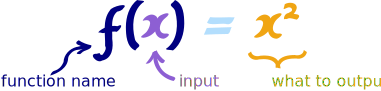
\includegraphics{images/function-fx-x2.svg}
\caption{alt text here}
\end{figure}

\begin{infobox}warning

A \textbf{mathematical function} is \ldots{}

an expression, rule, or law that defines a relationship between one variable (the \textbf{independent variable}, on the x-axis) and another variable (the \textbf{dependent variable}, on the y-axis).

\end{infobox}

From looking at the graph, here are two suggestions:

\[\begin{align}
\text{price} = 80 + 0.5 \cdot \text{age} \tag{Suggestion 1} \\
\text{price} = 90 + 0.2 \cdot \text{age} \tag{Suggestion 2} \\
\end{align}\]

\begin{infobox}warning

A \textbf{linear function} is \ldots{}

defined by two components, \textbf{intercept} (with the y-axis) and it's \textbf{slope}.

\end{infobox}

\begin{center}\includegraphics{Becoming-Fluent-In-Data_files/figure-latex/unnamed-chunk-105-1} \end{center}

\begin{infobox}warning
How can we compare the two suggested lines? Which linear function represents the relationship best?

\end{infobox}

\hypertarget{nobodys-perfect}{%
\subsection{Nobody's perfect}\label{nobodys-perfect}}

We all make mistakes. So do the linear functions:

\[ \begin{align}
\text{price} = 80 + 0.5 \cdot \text{age} \tag{Suggestion 1} \\
101 = 80 + 0.5 \cdot 42 \tag{Calculation for Hohlbein} \\
\end{align}\]

The equation tells (or predicts) that for any artist at the age of 42 it expects a auction price for a painting of 101 million US Dollar. Darmstadt Madonna was sold for 85 million US dollar. The linear function overestimated the true value. When you look at the graph, you see some predictions are more accurate (close to the true values) than others. All are either above or below the line.

\begin{infobox}warning

A \textbf{residual} (or error) is \ldots{}

the vertical distance between the actual and the predicted value.

\end{infobox}

\includegraphics{Becoming-Fluent-In-Data_files/figure-latex/unnamed-chunk-106-1.pdf}

\hypertarget{vocab-wrap-up}{%
\subsection{Vocab Wrap-Up}\label{vocab-wrap-up}}

Let's wrap up our regression vocab! We want to find an equation that describes the phenomenon of interest:

\[ \begin{align}
\text{outcome} &= f(\text{explanatory}) + \text{noise} \tag{Generic statistical model} \\
\text{outcome} &= \text{intercept} + \text{slope} \cdot \text{explanatory} + \text{noise} \tag{Generic linear model} \\
\end{align}\]

A \textbf{regression model} is suggested by the researcher. A more concrete regression model looks like this:

\[Y = \beta_1 + \beta_2 X + \epsilon\]

A model can be easy or complicated. It definitely contains variables and parameters.

\begin{itemize}
\tightlist
\item
  \textbf{Variables}: Things that we measure (or have data).
\item
  \textbf{Parameters}: Constant values we believe to represent some fundamental truth about the relationship between the variables.
\end{itemize}

What we (i.e.~the statistical software) actual do is an \textbf{estimation}. In textbooks the same equation can be found with hats:

\[   \widehat{Y}  = \widehat{\beta}_1 + \widehat{\beta}_2 \cdot X \]
\(\widehat{Y}\) are called the \textbf{fitted or predicted} values. \(\widehat{\beta}\) are \textbf{regression coefficients} (this is the estimate of the unknown population parameter). As we have seen in the graph before, the differences between the actual and the predicted values are the residuals \(e = Y - \widehat{Y}\).

\hypertarget{for-the-truly-dedicated}{%
\section{For the truly dedicated}\label{for-the-truly-dedicated}}

\begin{infobox}warning

Now we have all the ingredients we need.

\emph{Let's get this party started!}

\begin{figure}
\centering
\includegraphics{https://media1.tenor.com/images/6519b006f53708454922375a82c23682/tenor.gif?itemid=15161860}
\caption{Carlton Dance}
\end{figure}

\end{infobox}

The overall goal is to make as little as possible mistakes! What kind of mistake? The deviation from the observed values! What could come to your mind is to \textbf{minimize the sum of all errors}:

\[\sum e \rightarrow \min\]
But wait, there is more. Is it fair to say that the sum should be small? Compare \textbf{The Scream} and \textbf{Meules}, their deviations are \(+17.5\) and \(-13.6\) (very similar). So taken these two together, there's almost not mistake! That is to say, positive and negative deviations cancel each other out. Thus we need one more twist in the story:

\[\sum e^2 \rightarrow \min\]

\begin{infobox}warning

The fitting procedure is \ldots{}

is called \textbf{ordinary least squares} (short OLS). The goal of OLS is to \textbf{minimize the residual sum of squares}.

\end{infobox}

\hypertarget{algebra}{%
\subsection{Algebra}\label{algebra}}

\begin{infobox}warning
Algebra comes from Arabic, meaning ``reunion of broken parts''. We often work with matrices and vectors.

\end{infobox}

Now let's put all the things together. By convention, the \emph{normal} version of a vector is a vertical list of numbers in big parentheses (column vector). Transpose is when we change the rows and columns. In order to square a vector we need the following:

\[\sum e^2 = e^T \cdot e \rightarrow \min\]
Let's introduce matrix notation (there are 6 observations and two parameters):

\[ \begin{align}
Y &= \beta_0 + \beta_1 X + \epsilon \tag{X is a variable, Y is a variable} \\
\begin{pmatrix} Y_1 \\ Y_2 \\ Y_3 \\ Y_5 \\ Y_6 \end{pmatrix} &= \begin{pmatrix} 1 & X_{11} \\ 1 & X_{12} \\ 1 & X_{13} \\ 1 & X_{14} \\ 1 & X_{15} \\ 1 & X_{16}   \end{pmatrix} \begin{pmatrix} \beta_1 \\ \beta_2 \end{pmatrix} + \begin{pmatrix} \epsilon_1 \\ \epsilon_2 \\ \epsilon_3 \\ \epsilon_4 \\ \epsilon_5 \\ \epsilon_6 \\ \end{pmatrix} \\
y &= X \beta + \epsilon \tag{X is a matrix, y is a vector}
\end{align}\]

The residual is \(e = y - X \beta\) which we can plug in our minimal sum of squares:

\[\begin{align}
    \sum e^2 &= e^T \cdot e \tag{short RSS}\\
    &= (y - X \beta )^T (y - X \beta) \tag{$(A+B)^T = A^T + B^T$}\\
    &= (y^T - X^T \beta^T) (y - X \beta) \\
    &= y^T y - y^T X \beta - X^T \beta^T y + X^T \beta^T X \beta \\
    &= y^2 \underbrace{- 2 \beta^T X^T y}_{??} + \beta^2 X^2  \\
\end{align}\]

Did you notice what happened in the middle? The transpose of the first term is equal to the second:

\[\begin{align}
    (y^T X \beta)^T = y X^T \beta^T
\end{align}\]

\hypertarget{analysis}{%
\subsection{Analysis}\label{analysis}}

\begin{infobox}warning
In Analysis we often work with functions.

\end{infobox}

Next, we are ready to \textbf{optimize}. Optimization (in math and economics) is done by \textbf{differentiation}:

\[\begin{align}
    \frac{\partial RSS}{\partial \beta} &= -2 X^T y + 2 \beta X^T X = 0 \tag{first derivative equal to zero} \\
    2 \beta X^T X &= 2 X^T y \tag{rearrange terms}\\
    \beta X^T X &= X^T y \tag{the "normal equation"} \\
    \beta &= (X^T X)^{-1} X^T y \tag{Bam}\\
\end{align}\]

\hypertarget{take-the-long-way-home}{%
\subsection{Take the Long Way Home}\label{take-the-long-way-home}}

\begin{infobox}warning

\emph{The computer does the magic for us.}

\begin{figure}
\centering
\includegraphics{https://thumbs.gfycat.com/RemorsefulFairIndianpangolin-max-1mb.gif}
\caption{Magic Alice}
\end{figure}

\end{infobox}

Those \(\beta\) coefficients are one of the most important regression results. Retrieve them step by step to enhance your understanding of the math and coding as the same time:

First, we retrieve matrix \texttt{X} from the data set:

\begin{Shaded}
\begin{Highlighting}[]
\NormalTok{X}
\end{Highlighting}
\end{Shaded}

\begin{verbatim}
##      [,1] [,2]
## [1,]    1   91
## [2,]    1   86
## [3,]    1   67
## [4,]    1   45
## [5,]    1   80
## [6,]    1   71
\end{verbatim}

Second, the transpose of \texttt{X} has two rows and six columns:

\begin{Shaded}
\begin{Highlighting}[]
\FunctionTok{t}\NormalTok{(X)}
\end{Highlighting}
\end{Shaded}

\begin{verbatim}
##      [,1] [,2] [,3] [,4] [,5] [,6]
## [1,]    1    1    1    1    1    1
## [2,]   91   86   67   45   80   71
\end{verbatim}

Next, calculate the square of the matrix (transpose times original):

\begin{Shaded}
\begin{Highlighting}[]
\FunctionTok{t}\NormalTok{(X)}\SpecialCharTok{\%*\%}\NormalTok{X}
\end{Highlighting}
\end{Shaded}

\begin{verbatim}
##      [,1]  [,2]
## [1,]    6   440
## [2,]  440 33632
\end{verbatim}

Then, the inverse of everything in parentheses (the above matrix product):

\begin{Shaded}
\begin{Highlighting}[]
\FunctionTok{solve}\NormalTok{(}\FunctionTok{t}\NormalTok{(X)}\SpecialCharTok{\%*\%}\NormalTok{X)}
\end{Highlighting}
\end{Shaded}

\begin{verbatim}
##             [,1]          [,2]
## [1,]  4.10546875 -0.0537109375
## [2,] -0.05371094  0.0007324219
\end{verbatim}

Next, the product of this inverse and the transpose:

\begin{Shaded}
\begin{Highlighting}[]
\FunctionTok{solve}\NormalTok{(}\FunctionTok{t}\NormalTok{(X)}\SpecialCharTok{\%*\%}\NormalTok{X) }\SpecialCharTok{\%*\%} \FunctionTok{t}\NormalTok{(X)}
\end{Highlighting}
\end{Shaded}

\begin{verbatim}
##             [,1]         [,2]         [,3]        [,4]         [,5]
## [1,] -0.78222656 -0.513671875  0.506835938  1.68847656 -0.191406250
## [2,]  0.01293945  0.009277344 -0.004638672 -0.02075195  0.004882813
##              [,6]
## [1,]  0.291992188
## [2,] -0.001708984
\end{verbatim}

Finally, we multiply the vector \(y\):

\begin{Shaded}
\begin{Highlighting}[]
\FunctionTok{solve}\NormalTok{(}\FunctionTok{t}\NormalTok{(X)}\SpecialCharTok{\%*\%}\NormalTok{X) }\SpecialCharTok{\%*\%} \FunctionTok{t}\NormalTok{(X) }\SpecialCharTok{\%*\%}\NormalTok{ y}
\end{Highlighting}
\end{Shaded}

\begin{verbatim}
##           [,1]
## [1,] 22.345215
## [2,]  1.165747
\end{verbatim}

There are two numbers. It's the \(\beta\) vector! The first entry is the \textbf{intercept} and the second is the \textbf{slope} of the linear function:

\[Price = 22.3452 + 1.1657 \cdot Age\]

\hypertarget{survival-of-the-fittest-line}{%
\section{Survival of the Fittest Line}\label{survival-of-the-fittest-line}}

\begin{infobox}warning
The above equation is the linear function that best describes the given data.

\end{infobox}

\includegraphics{Becoming-Fluent-In-Data_files/figure-latex/unnamed-chunk-114-1.pdf}

\hypertarget{on-the-shoulders-of-giants}{%
\section{On the Shoulders of Giants}\label{on-the-shoulders-of-giants}}

Fortunately, we are \href{https://en.wikipedia.org/wiki/Standing_on_the_shoulders_of_giants}{standing on the shoulders of giants}. Clever people implemented the linear regression and all kinds of regressions and statistical tests in R.

\begin{Shaded}
\begin{Highlighting}[]
\FunctionTok{lm}\NormalTok{(Price }\SpecialCharTok{\textasciitilde{}}\NormalTok{ Age.at.Death, }\AttributeTok{data =}\NormalTok{ artists)}
\end{Highlighting}
\end{Shaded}

\begin{verbatim}
## 
## Call:
## lm(formula = Price ~ Age.at.Death, data = artists)
## 
## Coefficients:
##  (Intercept)  Age.at.Death  
##       22.345         1.166
\end{verbatim}

\includegraphics{images/workhorse.jpg}

  \bibliography{book.bib,packages.bib}

\end{document}
